Mucho del material de este capítulo es tomado de 
\cite{PRP},
\cite{RPL},
\cite{metaprogramming}
y de
\cite{ER}.

\begin{itemize}
\item
La \cei{metaprogramación} consiste en escribir programas y frameworks que nos ayudan a escribir programas
\item
La Wikipedia dice:

\begin{quote}
\wikip{Metaprogramming}{Metaprogramming} is the writing of computer programs that write or manipulate other programs (or themselves) as their data
\end{quote}
\item
The language in which the metaprogram is written is called the \cei{metalanguage} 
\item
The language of the programs that are manipulated is called the \cei{object language} 
\item
The ability of a programming language to
be its own metalanguage is called \cei{reflection} or \cei{reflexivity}
\item
Metaprogramación es un conjunto de técnicas que permiten extender la sintáxis de Ruby para hacer mas fácil la programación
\item
La metaprogramación esta fuertemente relacionada con la idea de escribir lenguajes de dominio específico (DSL)s (piensa en \rake{}, \rspec{}, \verb|Gemfile|, etc.)
\end{itemize}

\section{Tipos, Clases y Módulos}

Los \cei{métodos introspectivos} mas usados son los que determinan el tipo de un objeto.

\begin{verbatim}
>> obj = [1, {:a => 2}]
=> [1, {:a=>2}]
>> obj.class                      # retorna la clase de un objeto
=> Array
>> obj.class.superclass           # retorna la superclase de un objeto
=> Object
>> obj.instance_of? Object        # determina si obj.class == Object
=> false
>> obj.instance_of? Array
=> true
>> obj.is_a? Object               # determina si obj es de una subclase de Object
=> true
>> obj.is_a? Array
=> true
>> obj.kind_of? Object            # kind_of? es un sinónimo de is_a?
=> true
>> Array === obj                  # equivalente a obj.is_a? Array
=> true
>> Object === obj
=> true
>> obj.respond_to? 'each'        # si tiene un método público o protected llamado 'each'
=> true                          # si se le pasa true como segundo argumento se comprueban
                                 # también los privados
>> Array.instance_methods(false) 
=> ["insert"
 "sort" "include?" "size" "&" "to_ary" "clear" "yaml_initialize" "shuffle"
 "replace" "pack" "zip" "flatten!" "to_s" "pop" "pretty_print_cycle" "hash"
 "cycle" "*" "indices" "nitems" "index" "collect" "+" "compact!"
 "last" "rassoc" "count" "drop" "delete" "delete_at" "combination" "collect!"
 "select" "each_index" "-" "flatten" "eql?" "fill" "length" "uniq!"
 "at" "choice" "reject!" "[]" "take" "inspect" "shift" "compact"
 "pretty_print" "[]=" "|" "find_index" "slice!" "each" "empty?" "transpose"
 "<<" "frozen?" "rindex" "map" "reverse_each" "reverse!" "to_a" "push"
 "uniq" "delete_if" "first" "product" "drop_while" "concat" "reject"
 "map!" "join" "slice" "indexes" "taguri" "<=>" "assoc" "fetch" "to_yaml"
 "==" "values_at" "permutation" "take_while" "unshift" "reverse"
 "sort!" "shuffle!"  "taguri="]
\end{verbatim}

  \subsection{Antepasados y Módulos}
  
Los siguientes métodos sirven para determinar que módulos han sido incluídos 
y cuales son los ancestros de una clase o módulo:
\begin{verbatim}
[~/chapter8ReflectionandMetaprogramming]$ cat ancestryAndModules.rb 
module A; end

module B; include A; end

class C; include B; end

if __FILE__ == $0
  puts C < B               # => true: C includes B
  puts B < A               # => true: B includes A
  puts C < A               # => true
  puts Fixnum < Integer    # => true: all fixnums are integers
  puts Integer <Comparable # => true: integers are comparable
  puts Integer < Fixnum    # => false: not all integers are fixnums
  puts (String < Numeric).inspect  # => nil: strings are not numbers
  
  puts A.ancestors.inspect         # => [A]
  puts B.ancestors.inspect         # => [B, A]
  puts C.ancestors.inspect         # => [C, B, A, Object, Kernel, BasicObject]
  puts String.ancestors.inspect    # => [String, Comparable, Object, Kernel, BasicObject]
 
  puts C.include?(B)       # => true
  puts C.include?(A)       # => true
  puts B.include?(A)       # => true
  puts A.include?(A)       # => false 
  puts A.include?(B)       # => false

  puts A.included_modules.inspect  # => []
  puts B.included_modules.inspect  # => [A]
  puts C.included_modules.inspect  # => [B, A, Kernel]
end
\end{verbatim}

\begin{itemize}
\item
El método \modulep{include} es un método de instancia público definido en la clase \Module{}
\item
El método \verb|include| es un método privado de \Module{}.
\begin{verbatim}
ruby-1.9.2-head :002 > Module.private_methods.select { |x| x=~ /include/ }
 => [:included, :include] 
\end{verbatim}
(Para mas información sobre \verb|include|, véase la sección \ref{subsection:colisiones})
\end{itemize}

\subsubsection{El método \objecti{extend} de la clase \Object{}}
\label{susubsection:extend}
\begin{exercise}
¿Es posible incorporar los métodos de clase definidos en un módulo dentro 
de una clase? ¿Cual es el resultado de la llamada de la línea 15 en el siguiente
programa?
\begin{verbatim}
[~/chapter8ReflectionandMetaprogramming]$ cat -n including_class_methods1.rb 
 1  module Tutu
 2    def self.tutu; "tutu"; end
 3  end
 4  
 5  class Chazam
 6    include Tutu
 7  end
 8  
 9  puts Chazam.ancestors.inspect # [Chazam, Tutu, Object, Kernel, BasicObject]
10  
11  chazam_eigenclass = class << Chazam; self; end
12  
13  puts chazam_eigenclass.ancestors.inspect # [Class, Module, Object, Kernel, BasicObject]
14  
15  Chazam.tutu
\end{verbatim}
\end{exercise}
La línea:

  \begin{latexonly}
    \begin{lstlisting}

  chazam_eigenclass = class << Chazam; self; end

    \end{lstlisting}
  \end{latexonly}
    \begin{rawhtml}
    <pre>
<span class="n">chazam_eigenclass</span> <span class="o">=</span> <span class="k">class</span> <span class="o">&lt;&lt;</span> <span class="no">Chazam</span><span class="p">;</span> <span class="nb">self</span><span class="p">;</span> <span class="k">end</span>
    </pre>
    \end{rawhtml}
  
obtiene una referencia al objeto que representa la \cei{singleton class}, \cei{eigenclass} o \cei{metaclass} 
de \verb|Chazam|. 
Es posible obtener mas directamente la eigenclass de una clase
usando el método \kerneli{singleton\_class} de \Kernel{}:
\begin{verbatim}
ruby-1.9.2-head :001 > class Tutu; end
 => nil 
ruby-1.9.2-head :002 > Tutu.singleton_class
 => #<Class:Tutu> 
\end{verbatim}

Si tiene dudas para responder al ejercicio, 
repase la Sección \emph{La Búsqueda por Métodos} \ref{section:la_busqueda_por_metodos}.

\begin{exercise}
¿Que hacen las líneas 6-8 en el siguiente código?
¿Donde esta siendo incluído el módulo \verb|Tutu|?
¿Cual es el resultado de la llamada de la línea 17 en el siguiente código?
\begin{verbatim}
[~/chapter8ReflectionandMetaprogramming]$ cat -n including_class_methods2.rb 
 1  module Tutu
 2    def tutu; puts "tutu"; end
 3  end
 4  
 5  class Chazam
 6    class << self
 7      include Tutu
 8    end
 9  end
10  
11  puts Chazam.ancestors.inspect # [Chazam, Tutu, Object, Kernel, BasicObject]
12  
13  chazam_eigenclass = class << Chazam; self; end
14  
15  puts chazam_eigenclass.ancestors.inspect # [ Tutu, Class, Module, Object, Kernel, BasicObject]
16  
17  Chazam.tutu
\end{verbatim}
\end{exercise}

\begin{itemize}
\item
El método \objecti{extend} de la clase \Object{} hace que todos los métodos de los módulos 
especificados se conviertan en \cei{métodos singleton} 
(Véase la sección \ref{section:singleton_y_eigenclass})
del objeto sobre el que se llama \objecti{extend}:
\begin{verbatim}
module Greeter; def hi; "hello"; end; end # A silly module
s = "string object"
s.extend(Greeter)       # Add hi as a singleton method to s
s.hi                    # => "hello"
\end{verbatim}
\item 
Si \objecti{extend} se llama sobre un objeto \Class{} los métodos se añaden como 
métodos de clase:
\begin{verbatim}
String.extend(Greeter)  # Add hi as a class method of String
String.hi               # => "hello"
\end{verbatim}
\item
El método \objecti{extend} de la clase \Object{} 
es simplemente una abreviación que incluye el módulo
en la \cei{singleton class} o \cei{eigenclass} del objeto receptor
\end{itemize}

\subsubsection{El Método \modulec{nesting} de la clase \Module{}}
\begin{itemize}
\item
El método \modulec{nesting} de la clase \Module{} retorna un array especificando el anidamiento
de módulos en el punto de llamada:
\begin{verbatim}
module M
  class C
    Module.nesting   # => [M::C, M]
  end
end
\end{verbatim}
\end{itemize}

  \subsection{Definiendo Clases y Módulos}

Las clases y los módulos son instancias de las clases \rubymod{Class} y \rubymod{Module}.
Por tanto, es posible crearlos dinámicamente:
\begin{verbatim}
M = Module.new      # Define a new module M
C = Class.new       # Define a new class C
D = Class.new(C) {  # Define a subclass of C
  include M         # that includes module M
}
D.to_s              # => "D": class gets constant name by magic
\end{verbatim}

Cuando un módulo o clase dinámicamente creado es asignado a una constante el nombre de esa 
constante es usado como nombre del módulo o clase.


\begin{verbatim}
~/Chapter8ReflectionandMetaprogramming$ cat -n dynamicclassesandmodules.rb 
     1  Fred = Module.new do
     2    def meth1
     3      "hello #{args.inspect}"
     4    end
     5    def meth2
     6      "bye #{args.inspect}"
     7    end
     8  end
     9  
    10  Klass = Class.new do
    11    include Fred
    12    attr_accessor 'args'
    13  
    14    def initialize(*args)
    15      @args = args
    16    end
    17  end
    18  
    19  puts Fred.to_s     # Fred
    20  puts Klass.name    # Klass
    21  
    22  a = Klass.new(4, 5)
    23  
    24  puts a.meth1     # hello [4, 5] 
    25  puts a.meth2     # bye [4, 5]
\end{verbatim}
\begin{itemize}
\item
Cuando una clase o módulo es creado dinámicamente y asignado a una constante, el nombre de la constante
es utilizado como nombre de la clase 

\item
Si fuera asignado a una
variable, el método \methodi{to\_s} devolvería algo del estilo
\verb|#<Class:0x10016a868>| y \modulei{name} devolvería \verb|nil|.
\end{itemize}

\subsubsection{\Class{}.new, \Module{}.new, \modulei{define\_method} y Ambitos}

\begin{enumerate}
\item 
El método \kerneli{local\_variables} del módulo \Kernel{} nos permite acceder
a las variables locales visibles en un punto.
\item 
Algunos lenguajes permiten a un \cei{ámbito} interno ver las variables
de un ámbito mas externo. Este tipo de visibilidad no ocurre en Ruby
\item 
Hay tres puntos en los que un programa abandona el ámbito previo y
abre un nuevo ámbito (\cei{scope gates} en al terminología del libro \emph{Metaprogramming Ruby}
\cite{metaprogramming}):
\begin{enumerate}
\item 
Definiciones de clase
\item 
Definiciones de módulo
\item 
Definiciones de método
\end{enumerate}
\item 
Las variables globales son visibles desde cualquier ámbito
\item 
las variables de instancia son visibles desde cualquier punto en el que 
\verb|self| se refiere al mismo objeto
\end{enumerate}


  \begin{latexonly}
    \begin{lstlisting}

  v1 = 1                  
  
  class Tutu
    v2 = 2                
    puts "%2d"%(__LINE__.to_s)+' '+local_variables.inspect # [:v2]
  
    def my_method
      v3 = 3
      puts "%2d"%__LINE__.to_s+' '+local_variables.inspect # [:v3]
    end
  
    puts "%2d"%__LINE__.to_s+' '+local_variables.inspect   # [:v2] 
  end
  
  obj = Tutu.new
  obj.my_method        
  obj.my_method        
  puts "%2d"%__LINE__.to_s+' '+local_variables.inspect     # [:v1, :obj]

    \end{lstlisting}
  \end{latexonly}
    \begin{rawhtml}
    <pre>
<span class="n">v1</span> <span class="o">=</span> <span class="mi">1</span>                  
  
  <span class="k">class</span> <span class="nc">Tutu</span>
    <span class="n">v2</span> <span class="o">=</span> <span class="mi">2</span>                
    <span class="nb">puts</span> <span class="s2">&quot;%2d&quot;</span><span class="sx">%(__LINE__.to_s)</span><span class="o">+</span><span class="s1">&#39; &#39;</span><span class="o">+</span><span class="nb">local_variables</span><span class="o">.</span><span class="n">inspect</span> <span class="c1"># [:v2]</span>
  
    <span class="k">def</span> <span class="nf">my_method</span>
      <span class="n">v3</span> <span class="o">=</span> <span class="mi">3</span>
      <span class="nb">puts</span> <span class="s2">&quot;%2d&quot;</span><span class="sx">%__</span><span class="no">LINE__</span><span class="o">.</span><span class="n">to_s</span><span class="o">+</span><span class="s1">&#39; &#39;</span><span class="o">+</span><span class="nb">local_variables</span><span class="o">.</span><span class="n">inspect</span> <span class="c1"># [:v3]</span>
    <span class="k">end</span>
  
    <span class="nb">puts</span> <span class="s2">&quot;%2d&quot;</span><span class="sx">%__</span><span class="no">LINE__</span><span class="o">.</span><span class="n">to_s</span><span class="o">+</span><span class="s1">&#39; &#39;</span><span class="o">+</span><span class="nb">local_variables</span><span class="o">.</span><span class="n">inspect</span>   <span class="c1"># [:v2] </span>
  <span class="k">end</span>
  
  <span class="n">obj</span> <span class="o">=</span> <span class="no">Tutu</span><span class="o">.</span><span class="n">new</span>
  <span class="n">obj</span><span class="o">.</span><span class="n">my_method</span>        
  <span class="n">obj</span><span class="o">.</span><span class="n">my_method</span>        
  <span class="nb">puts</span> <span class="s2">&quot;%2d&quot;</span><span class="sx">%__</span><span class="no">LINE__</span><span class="o">.</span><span class="n">to_s</span><span class="o">+</span><span class="s1">&#39; &#39;</span><span class="o">+</span><span class="nb">local_variables</span><span class="o">.</span><span class="n">inspect</span>     <span class="c1"># [:v1, :obj]</span>
    </pre>
    \end{rawhtml}
  

Puesto que \Class{}.new, \Module{}.new y \modulei{define\_method}
usan el bloque que les sigue y los bloques no abandonan el \cei{ámbito} previo (aunque 
crean uno nuevo),
podemos jugar con estos tres métodos para crear clausuras en las que se comparten
variables locales entre clases, métodos y ámbitos. Observe como en esta
reescritura del programa anterior cambia la visibilidad:


  \begin{latexonly}
    \begin{lstlisting}

  v1 = 1                  
  
  Tutu = Class.new do
    v2 = 2                
    puts "%2d"%(__LINE__.to_s)+' '+local_variables.inspect  # [:v2, :v1, :obj]
  
    define_method :my_method  do
      v3 = 3
      puts "%2d"%__LINE__.to_s+' '+local_variables.inspect  # [:v3, :v2, :v1, :obj]
    end
  
    puts "%2d"%__LINE__.to_s+' '+local_variables.inspect    # [:v2, :v1, :obj]
  end
  
  obj = Tutu.new
  obj.my_method        
  obj.my_method        
  puts "%2d"%__LINE__.to_s+' '+local_variables.inspect       # [:v1, :obj]

    \end{lstlisting}
  \end{latexonly}
    \begin{rawhtml}
    <pre>
<span class="n">v1</span> <span class="o">=</span> <span class="mi">1</span>                  
  
  <span class="no">Tutu</span> <span class="o">=</span> <span class="no">Class</span><span class="o">.</span><span class="n">new</span> <span class="k">do</span>
    <span class="n">v2</span> <span class="o">=</span> <span class="mi">2</span>                
    <span class="nb">puts</span> <span class="s2">&quot;%2d&quot;</span><span class="sx">%(__LINE__.to_s)</span><span class="o">+</span><span class="s1">&#39; &#39;</span><span class="o">+</span><span class="nb">local_variables</span><span class="o">.</span><span class="n">inspect</span>  <span class="c1"># [:v2, :v1, :obj]</span>
  
    <span class="n">define_method</span> <span class="ss">:my_method</span>  <span class="k">do</span>
      <span class="n">v3</span> <span class="o">=</span> <span class="mi">3</span>
      <span class="nb">puts</span> <span class="s2">&quot;%2d&quot;</span><span class="sx">%__</span><span class="no">LINE__</span><span class="o">.</span><span class="n">to_s</span><span class="o">+</span><span class="s1">&#39; &#39;</span><span class="o">+</span><span class="nb">local_variables</span><span class="o">.</span><span class="n">inspect</span>  <span class="c1"># [:v3, :v2, :v1, :obj]</span>
    <span class="k">end</span>
  
    <span class="nb">puts</span> <span class="s2">&quot;%2d&quot;</span><span class="sx">%__</span><span class="no">LINE__</span><span class="o">.</span><span class="n">to_s</span><span class="o">+</span><span class="s1">&#39; &#39;</span><span class="o">+</span><span class="nb">local_variables</span><span class="o">.</span><span class="n">inspect</span>    <span class="c1"># [:v2, :v1, :obj]</span>
  <span class="k">end</span>
  
  <span class="n">obj</span> <span class="o">=</span> <span class="no">Tutu</span><span class="o">.</span><span class="n">new</span>
  <span class="n">obj</span><span class="o">.</span><span class="n">my_method</span>        
  <span class="n">obj</span><span class="o">.</span><span class="n">my_method</span>        
  <span class="nb">puts</span> <span class="s2">&quot;%2d&quot;</span><span class="sx">%__</span><span class="no">LINE__</span><span class="o">.</span><span class="n">to_s</span><span class="o">+</span><span class="s1">&#39; &#39;</span><span class="o">+</span><span class="nb">local_variables</span><span class="o">.</span><span class="n">inspect</span>       <span class="c1"># [:v1, :obj]</span>
    </pre>
    \end{rawhtml}
  

\section{Evaluando Strings y Bloques}

El método \kerneli{eval}  de \Kernel{}
permite evaluar el código contenido en un objeto \rubymod{String}:
\begin{verbatim}
>> x = 1
=> 1
>> eval "x+1"
=> 2
\end{verbatim}

en general, se desaconseja 
el uso de \verb|eval| cuando se trabaja en una aplicación 
distribuída en la que los datos pueden venir de fuentes externas.

  \subsection{Bindings (encarpetados) y eval}
   
\begin{enumerate}
\item 
Un \rubymod{Binding} es un objeto que representa el estado de los bindings 
definidos por las variables en un instante dado.

\item 
El método \kerneli{binding} retorna un objeto \Binding{} describiendo
los bindings en efecto en el punto de la llamada.

\item 
Es posible pasarle a \kerneli{eval}
un segundo argumento de la clase \rubymod{Binding}
que especifique el contexto en que es evaluada la cadena:
\end{enumerate}
\begin{verbatim}
~/Chapter8ReflectionandMetaprogramming$ cat -n bindingsAndEval.rb 
     1  class Demo
     2    def initialize(n)
     3      @secret = n
     4    end
     5    def getBinding
     6      return binding()
     7    end
     8  end
     9  
    10  k1 = Demo.new(99)
    11  b1 = k1.getBinding
    12  k2 = Demo.new(-3)
    13  b2 = k2.getBinding
    14  
    15  puts eval("@secret", b1)   #=> 99
    16  puts eval("@secret", b2)   #=> -3
    17  puts eval("@secret")       #=> nil
\end{verbatim}
Ejecución:
\begin{verbatim}
~/Chapter8ReflectionandMetaprogramming$ ruby bindingsAndEval.rb 
99
-3
nil

\end{verbatim}

\subsubsection{Procs y Bindings}

\begin{enumerate}
\item 
La clase \rubymod{Proc} define un método \proci{binding}.
Cuando se llama dentro de un proc o de una lambda retorna un objeto 
\rubymod{Binding} que representa los bindings en efecto en la clausura
de ese \Proc{}.

\item 
Además, el método de \Kernel{} \kerneli{eval} nos permite pasar como segundo argumento un \Proc{} en vez de un \Binding{}
(Véase la sección \ref{subsection:clausurasybindings}).

\item 
Además, Ruby 1.9 define un método \bindingi{eval} para los objetos \Binding{}.
\end{enumerate}


  \begin{latexonly}
    \begin{lstlisting}

      def fred(param)
        proc {}
      end
      
      def multiplier(n)
        lambda do |*arr| 
                  arr.collect { |i| i*n } 
               end
      end
      
      b = fred(99)
      puts eval("param", b.binding)   #=> 99
      puts eval("param", b)           #=> 99
      
      puts "********************************"
      doubler = multiplier(2)
      puts doubler[1, 2, 3] # 2 4 6
      
      puts "********************************"
      eval("n = 3", doubler.binding)
      puts doubler.call(1, 2, 3) # 3 6 9
      
      puts "********************************"
      eval("n = 5", doubler)
      puts doubler.call(1, 2, 3) # 5 10 15

    \end{lstlisting}
  \end{latexonly}
    \begin{rawhtml}
    <pre>
<span class="k">def</span> <span class="nf">fred</span><span class="p">(</span><span class="n">param</span><span class="p">)</span>
        <span class="nb">proc</span> <span class="p">{}</span>
      <span class="k">end</span>
      
      <span class="k">def</span> <span class="nf">multiplier</span><span class="p">(</span><span class="n">n</span><span class="p">)</span>
        <span class="nb">lambda</span> <span class="k">do</span> <span class="o">|*</span><span class="n">arr</span><span class="o">|</span> 
                  <span class="n">arr</span><span class="o">.</span><span class="n">collect</span> <span class="p">{</span> <span class="o">|</span><span class="n">i</span><span class="o">|</span> <span class="n">i</span><span class="o">*</span><span class="n">n</span> <span class="p">}</span> 
               <span class="k">end</span>
      <span class="k">end</span>
      
      <span class="n">b</span> <span class="o">=</span> <span class="n">fred</span><span class="p">(</span><span class="mi">99</span><span class="p">)</span>
      <span class="nb">puts</span> <span class="nb">eval</span><span class="p">(</span><span class="s2">&quot;param&quot;</span><span class="p">,</span> <span class="n">b</span><span class="o">.</span><span class="n">binding</span><span class="p">)</span>   <span class="c1">#=&gt; 99</span>
      <span class="nb">puts</span> <span class="nb">eval</span><span class="p">(</span><span class="s2">&quot;param&quot;</span><span class="p">,</span> <span class="n">b</span><span class="p">)</span>           <span class="c1">#=&gt; 99</span>
      
      <span class="nb">puts</span> <span class="s2">&quot;********************************&quot;</span>
      <span class="n">doubler</span> <span class="o">=</span> <span class="n">multiplier</span><span class="p">(</span><span class="mi">2</span><span class="p">)</span>
      <span class="nb">puts</span> <span class="n">doubler</span><span class="o">[</span><span class="mi">1</span><span class="p">,</span> <span class="mi">2</span><span class="p">,</span> <span class="mi">3</span><span class="o">]</span> <span class="c1"># 2 4 6</span>
      
      <span class="nb">puts</span> <span class="s2">&quot;********************************&quot;</span>
      <span class="nb">eval</span><span class="p">(</span><span class="s2">&quot;n = 3&quot;</span><span class="p">,</span> <span class="n">doubler</span><span class="o">.</span><span class="n">binding</span><span class="p">)</span>
      <span class="nb">puts</span> <span class="n">doubler</span><span class="o">.</span><span class="n">call</span><span class="p">(</span><span class="mi">1</span><span class="p">,</span> <span class="mi">2</span><span class="p">,</span> <span class="mi">3</span><span class="p">)</span> <span class="c1"># 3 6 9</span>
      
      <span class="nb">puts</span> <span class="s2">&quot;********************************&quot;</span>
      <span class="nb">eval</span><span class="p">(</span><span class="s2">&quot;n = 5&quot;</span><span class="p">,</span> <span class="n">doubler</span><span class="p">)</span>
      <span class="nb">puts</span> <span class="n">doubler</span><span class="o">.</span><span class="n">call</span><span class="p">(</span><span class="mi">1</span><span class="p">,</span> <span class="mi">2</span><span class="p">,</span> <span class="mi">3</span><span class="p">)</span> <span class="c1"># 5 10 15</span>
    </pre>
    \end{rawhtml}
  

ejecución:
\begin{verbatim}
~/Chapter8ReflectionandMetaprogramming$ ruby procsAndBindings.rb 
99
99
********************************
2
4
6
********************************
3
6
9
********************************
5
10
15
\end{verbatim}

  \subsection{instance\_eval y class\_eval}

\begin{itemize}
\item
La clase \rubymod{BasicObject} define el método \basicobjecti{instance\_eval}.
\begin{verbatim}
ruby-1.9.2-head :004 > BasicObject.public_methods.select { |x| x =~ /instance_e/ }
 => [:instance_eval, :instance_exec] 
\end{verbatim}
\item
La clase \rubymod{Module} define el método \modulei{class\_eval}.
\item El método \modulei{module\_eval} es un sinónimo de \modulei{class\_eval}.
\end{itemize}
Estos dos métodos evaluan de manera similar a \verb|eval| pero con estas consideraciones:
\begin{enumerate}
\item Evaluan el código en el contexto del objeto o de la clase o módulo especificados
\item El objeto o módulo es el valor de \verb|self| durante la evaluación
\item
\basicobjecti{instance\_eval} define métodos singleton del objeto 
(y, por tanto define métodos de clase cuando el objeto es una clase)
\begin{verbatim}
# Use instance_eval to define class method String.empty
# Note that quotes within quotes get a little tricky...
String.instance_eval("def empty; ''; end")
\end{verbatim}
\item
\modulei{class\_eval} define métodos de instancia 
\begin{verbatim}
# Define an instance method len of String to return string length
String.class_eval("def len; size; end")
\end{verbatim}
\item \objecti{instance\_eval} y  \modulei{class\_eval} aceptan un bloque de código como argumento para la evaluación
\begin{verbatim}
String.class_eval {
  def len
    size
  end
}
String.class_eval { alias len size }
String.instance_eval { def empty; ""; end }
\end{verbatim}

\item
La sintáxis de \basicobjecti{instance\_eval} es:
\begin{verbatim}
    instance_eval(string [, filename [, lineno]] ) 
    instance_eval {| | block } 
\end{verbatim}
En el caso de la \String{}, los dos últimos argumentos 
son utilizados para mejorar los mensajes de error
\item
El método \modulei{class\_eval} tiene la sintaxis:

\begin{verbatim}
class_eval(string [, filename [, lineno]])
module_eval {|| block }
\end{verbatim}
\end{enumerate}
Veamos un ejemplo:


  \begin{latexonly}
    \begin{lstlisting}

    class Klass
      def initialize
        @secret = 99
      end
    end
    k = Klass.new
    k2 = Klass.new
    puts k.instance_eval { @secret }   #=> 99
    
    k.instance_eval " def tutu; puts self.inspect; %q{hello}; end"  
    puts k.tutu    # #<Klass:0x10016a9f8 @secret=99> 
                   # hello
    begin
      puts k2.tutu   # "tutu" is a singleton method of "k"
    rescue NoMethodError
      puts $!  # undefined method `tutu' for #<Klass:0x10016a958 @secret=99>
    end
    
    Klass.instance_eval {
      def chachi     # A singleton method of a class is a class method!
        self.inspect
      end
    }
    
    puts Klass.chachi # Klass

    \end{lstlisting}
  \end{latexonly}
    \begin{rawhtml}
    <pre>
<span class="k">class</span> <span class="nc">Klass</span>
      <span class="k">def</span> <span class="nf">initialize</span>
        <span class="vi">@secret</span> <span class="o">=</span> <span class="mi">99</span>
      <span class="k">end</span>
    <span class="k">end</span>
    <span class="n">k</span> <span class="o">=</span> <span class="no">Klass</span><span class="o">.</span><span class="n">new</span>
    <span class="n">k2</span> <span class="o">=</span> <span class="no">Klass</span><span class="o">.</span><span class="n">new</span>
    <span class="nb">puts</span> <span class="n">k</span><span class="o">.</span><span class="n">instance_eval</span> <span class="p">{</span> <span class="vi">@secret</span> <span class="p">}</span>   <span class="c1">#=&gt; 99</span>
    
    <span class="n">k</span><span class="o">.</span><span class="n">instance_eval</span> <span class="s2">&quot; def tutu; puts self.inspect; %q{hello}; end&quot;</span>  
    <span class="nb">puts</span> <span class="n">k</span><span class="o">.</span><span class="n">tutu</span>    <span class="c1"># #&lt;Klass:0x10016a9f8 @secret=99&gt; </span>
                   <span class="c1"># hello</span>
    <span class="k">begin</span>
      <span class="nb">puts</span> <span class="n">k2</span><span class="o">.</span><span class="n">tutu</span>   <span class="c1"># &quot;tutu&quot; is a singleton method of &quot;k&quot;</span>
    <span class="k">rescue</span> <span class="no">NoMethodError</span>
      <span class="nb">puts</span> <span class="vg">$!</span>  <span class="c1"># undefined method `tutu&#39; for #&lt;Klass:0x10016a958 @secret=99&gt;</span>
    <span class="k">end</span>
    
    <span class="no">Klass</span><span class="o">.</span><span class="n">instance_eval</span> <span class="p">{</span>
      <span class="k">def</span> <span class="nf">chachi</span>     <span class="c1"># A singleton method of a class is a class method!</span>
        <span class="nb">self</span><span class="o">.</span><span class="n">inspect</span>
      <span class="k">end</span>
    <span class="p">}</span>
    
    <span class="nb">puts</span> <span class="no">Klass</span><span class="o">.</span><span class="n">chachi</span> <span class="c1"># Klass</span>
    </pre>
    \end{rawhtml}
  

Los dos últimos argumentos 
\verb|class_eval(string [, filename [, lineno]])|
son utilizados para mejorar los mensajes de error:

\begin{verbatim}
~/Chapter8ReflectionandMetaprogramming$ cat -n class_eval.rb 
     1  class Thing
     2  end
     3  a = %q{def hello() "Hello there!" end}
     4  Thing.module_eval(a)
     5  puts Thing.new.hello()
     6                                     
     7  Thing.module_eval("invalid code", 
     8                    "ficherito.rb", 
     9                    123               # nº de linea
    10                   )
\end{verbatim}
Ejecución:
\begin{verbatim}
~/Chapter8ReflectionandMetaprogramming$ ruby class_eval.rb 
Hello there!
ficherito.rb:123: undefined local variable or method `code' for Thing:Class (NameError)
\end{verbatim}


\subsubsection{Creando accessors con class\_eval}
Sabemos que podemos crear accessors a los atributos de una clase
usando \verb|attr_accessor|, \verb|attr_reader| y \verb|attr_writer|.
Estas no son palabras reservadas de Ruby sino que se trata de métodos.
Veamos como podemos emular su construcción  usando \modulei{class\_eval}:

\begin{verbatim}
MacBookdeCasiano:chapter8ReflectionandMetaprogramming casiano$ cat -n myAccessors.rb 
     1  class Module
     2    def my_attr_reader(*syms) # método de instancia de Module
     3      syms.each { |s|         # esto es, ¡un método de clase!
     4        class_eval %{         # aquí self es el objeto Module
     5                      def #{s}  # estamos definiendo un método de 
     6                        @#{s}   #instancia en la clase "self"
     7                      end
     8                    }
     9      }
    10    end
    11  end
    12  
    13  class Chuchu
    14    my_attr_reader :a, :b
    15  
    16    def initialize(a,b)
    17      @a, @b = a, b
    18    end
    19  end
    20  
    21  x = Chuchu.new(4, "z")
    22  puts x.a    # 4
    23  puts x.b    # z
\end{verbatim}

  \subsection{instance\_exec y class\_exec}
Los métodos
\basicobjecti{instance\_exec} (\BasicObject{})
y 
\modulei{class\_exec} 
(y su alias \modulei{module\_exec}, ambos en \Module{})
evaluan un bloque 
(pero no una \String{})
de la misma forma que sus homólogos \basicobjecti{instance\_eval}
y \modulei{class\_eval}.
La diferencias es que los métodos \verb|exec| aceptan argumentos
que pasan al bloque evaluado.

\section{Variables y Constantes}

Existen métodos para listar los nombres (como cadenas)
de 
\begin{itemize}
\item las variables globales que estén definidas (\kerneli{global\_variables}, definido en \Kernel{}) 
\item de las variables locales que estén actualmente definidas (\kerneli{local\_variables}, definido en \Kernel{})
\item de las variables de instancia de un objeto (\objecti{instance\_variables}, definido en \Object{})
\item de las variables de clase o módulo (\classi{class\_variables}, definido en \Class{})
\item y de las constantes de una clase o módulo (\modulei{constants}, definido en \Module{})
\end{itemize}

\begin{verbatim}
~/chapter8ReflectionandMetaprogramming$ cat -n variablesAndConstants.rb 
 1  class Tutu
 2    def initialize(x,y); @x, @y = x, y; end
 3    @@classvar = 1
 4    ORIGIN = Tutu.new(0, 0)
 5  end
 6  
 7  puts "Globals variables with 'D': "
 8  puts("  "+global_variables.select { |w| w =~/D/ }.inspect) #  [:$KCODE, :$LOAD_PATH, :$LOADED_FEATURES, :$DEBUG]
 9  x = 1
10  puts "Local variables:"
11  puts "  #{local_variables.inspect}" # [:x]
12  
13  puts "Instance variable names: "
14  Tutu::ORIGIN.instance_variables.each { |v|
15    puts "  #{v}"                     #   @x @y
16  }
17  puts "Class variables names: "
18  Tutu.class_variables.each { |v|
19    puts "  #{v}"                     # @@classvar
20  }
21  puts "Constant names: "
22  Tutu.constants.each { |c|
23    puts "  #{c}"                     # ORIGIN
24  }
\end{verbatim}
Ejecución:
\begin{verbatim}
~/chapter8ReflectionandMetaprogramming$ ruby variablesAndConstants.rb 
Globals variables with 'D': 
  ["$KCODE", "$LOAD_PATH", "$DEBUG", "$LOADED_FEATURES"]
Local variables:
  ["x"]
Instance variable names: 
  @x
  @y
Class variables names: 
  @@classvar
Constant names: 
  ORIGIN
\end{verbatim}

\subsection{Buscando, Dando Valores y Suprimiendo Variables y Constantes}

No existen métodos especiales para indagar o dar valores a las variables
locales y globales pero siempre es posible usar \kerneli{eval} para eso:
\begin{verbatim}
x = 1
varname = "x"
eval(varname)           # => 1
eval("varname = '$g'")  # Set varname to "$g"
eval("#{varname} = x")  # Set $g to 1
eval(varname)           # => 1
\end{verbatim}
Cualesquiera variables que
se definen dentro de un \verb|eval| son locales al \verb|eval|
ydejan de existir cuando este retorna.

Es posible preguntar por el valor, poner el valor y comprobar la existencia
de variables de instancia de cualquier objeto y de variables y constantes de 
clase (o módulo):
\begin{verbatim}
o = Object.new
o.instance_variable_set(:@x, 0)   # Note required @ prefix
o.instance_variable_get(:@x)      # => 0
o.instance_variable_defined?(:@x) # => true

Object.class_variable_set(:@@x, 1)   # Private in Ruby 1.8
Object.class_variable_get(:@@x)      # Private in Ruby 1.8
Object.class_variable_defined?(:@@x) # => true; Ruby 1.9 and later

Math.const_set(:EPI, Math::E*Math::PI)
Math.const_get(:EPI)             # => 8.53973422267357
Math.const_defined? :EPI         # => true 
\end{verbatim}

\begin{verbatim}
String.class_eval { class_variable_set(:@@x, 1) }  # Set @@x in String
String.class_eval { class_variable_get(:@@x) }     # => 1
\end{verbatim}

\begin{verbatim}
o.instance_eval { remove_instance_variable :@x }
String.class_eval { remove_class_variable(:@@x) }
Math.send :remove_const, :EPI  # Use send to invoke private method
\end{verbatim}

\begin{verbatim}
def Symbol.const_missing(name)
  name # Return the constant name as a symbol
end
Symbol::Test   # => :Test: undefined constant evaluates to a Symbol
\end{verbatim}

\section{Métodos}

\subsection{Listando y Comprobando Métodos}

\subsection{Obteniendo los Métodos de Objetos}

\subsection{Llamando a los Métodos Dinámicamente}
Cuando llamamamos a un método, usamos la notación \I{punto}.
Sin embargo, también podemos usar el método \verb|send| de la clase
\rubymod{Object}:
\begin{verbatim}
MacBookdeCasiano:chapter8ReflectionandMetaprogramming casiano$ cat -n dynamiccall.rb 
     1  class Tutu
     2    def tutu(arg)
     3      a = arg*2
     4      yield a if block_given?
     5    end
     6  end
     7  
     8  obj = Tutu.new
     9  obj.tutu(4) { |m| puts "In block: #{m}" }
    10  print "Action?: "
    11  n = gets.chomp!.to_sym 
    12  obj.send(n, 5) { |m| puts "In block: #{m}" }
\end{verbatim}
Ejecución:

\begin{verbatim}
MacBookdeCasiano:chapter8ReflectionandMetaprogramming casiano$ ruby dynamiccall.rb 
In block: 8
Action?: tutu
In block: 10
\end{verbatim}

\subsubsection{send: Rendimiento}
El módulo \rubystdlibclass{Benchmark}{benchmark/rdoc/Benchmark} nos permite comparar el rendimiento de distintos códigos:
\begin{verbatim}
~/rubytesting$ cat -n benchcall.rb 
     1  require 'benchmark' 
     2  include Benchmark
     3  test = "Comparing Calls" 
     4  m = test.method(:length) 
     5  n = 1000000
     6  bm(12) {|x| 
     7    x.report("call") { n.times { m.call             } } 
     8    x.report("send") { n.times { test.send(:length) } }
     9    x.report("eval") { n.times { eval "test.length" } }
    10  }
\end{verbatim}

\begin{verbatim}
~/rubytesting$ ruby benchcall.rb 
                  user     system      total        real
call          0.210000   0.000000   0.210000 (  0.209029)
send          0.240000   0.000000   0.240000 (  0.247114)
eval          1.950000   0.000000   1.950000 (  1.951107)
\end{verbatim}

\subsection{Definiendo, Suprimiendo y Haciendo Alias de Métodos}

\subsubsection{Definiendo Métodos con define\_method}
%Ruby uses two ways to generate methods dynamically; define_method (on the left) and the (older) class_eval + def (right box). First, a quick snapshot of the API: 
%      
En Ruby tenemos dos formas de generar métodos 
dinámicamente: \verb|define_method| y
\verb|eval + def|. 
\begin{tabular}{|p{6cm}|p{6cm}|}
\begin{verbatim}
define_method(symbol, method)

\end{verbatim}
&
\begin{verbatim}
define_method(symbol) { block }  

 class_eval <<-"END"
  def #{name}
    # body 
  end  
 END
\end{verbatim}
\end{tabular}
\verb|define_method| es un método de clase privado y por tanto debe ser invocado sin especificar 
el receptor: el destinatario es siempre la clase que esta en contexto.
Los parámetros son:

\begin{itemize}
\item
\verb|symbol| especifica el nombre del método. 
\item
\verb|method| es una \verb|lambda| o \verb|Proc| o un bloque.
\end{itemize}

\begin{verbatim}
~/chapter8ReflectionandMetaprogramming$ cat -n hashtoclass.rb 
     1  class MyClass 
     2      def self.h; @@h end
     3  
     4      print "Write a ruby hash: "
     5      @@h = eval gets() 
     6  
     7      @@h.keys.each { |k|
     8        define_method k do
     9         @@h[k] 
    10        end
    11  
    12        define_method "#{k}=" do |v|
    13         @@h[k] = v 
    14        end
    15      }
    16  end
    17  
    18  x = MyClass.new
    19  print "Action: "; action = gets().chomp
    20  if action =~ /=/
    21    print "Value: "; value = eval gets().chomp
    22    puts x.send(action, value)
    23  else 
    24    puts x.send(action)
    25  end
    26  puts MyClass.h.inspect
\end{verbatim}

\begin{verbatim}
~/chapter8ReflectionandMetaprogramming$ ruby hashtoclass.rb 
Write a ruby hash: { :a => 1, :b => 2}
Action: b=
Value: 45
45
{:a=>1, :b=>45}
\end{verbatim}

\verb|define_method| nos permite definir métodos cuyos nombres no se atienen a las reglas convencionales:

\begin{verbatim}
>> class Titi
>> define_method 'chu$|chu' do
?> puts "in chu$|chu"
>> end
>> end
=> #<Proc:0x000000010046d8f8@(irb):33>
>> z = Titi.new
=> #<Titi:0x10046ac20>
>> z.send 'chu$|chu'
in chu$|chu
=> nil
\end{verbatim}

\subsection{Manejando Métodos No Definidos: method\_missing}
\label{seubsection:methodmissing}
\begin{verbatim}
MacBookdeCasiano:rubytesting casiano$ cat -n searchmethod.rb 
     1  class A
     2    def tutu
     3      puts "A::tutu"
     4    end
     5    def method_missing(name, *args)
     6      puts "In A::method missing"
     7    end
     8  end
     9  
    10  class B < A
    11    def method_missing(name, *args)
    12      puts "In B::method missing"
    13    end
    14  end
    15  
    16  x = B.new
    17  x.tutu()    # A::tutu
    18  
    19  y = A.new
    20  y.titi()    # In A::method missing
    21  
    22  z = B.new   # In B::method missing
    23  z.tete()
\end{verbatim}

\begin{verbatim}
MacBookdeCasiano:rubytesting casiano$ ruby searchmethod.rb 
A::tutu
In A::method missing
In B::method missing
\end{verbatim}

\begin{verbatim}
~/chapter8ReflectionandMetaprogramming$ cat -n method_missing.rb 
     1  class Shell
     2    def method_missing(method, *args)
     3      r = %x{#{method} #{args.join(' ')} 2>&1}
     4      return r unless block_given?
     5      yield r 
     6    end
     7  end
     8  
     9  s = Shell.new
    10  puts s.ls('-l', 'r*.rb') { |x|
    11    puts "inside block" 
    12    x.gsub(/^/,'** ')
    13  }
    14  puts s.uname
\end{verbatim}

\begin{verbatim}
~/chapter8ReflectionandMetaprogramming$ ruby method_missing.rb 
inside block
** -rw-r--r--  1 casianorodriguezleon  staff  1195  1 nov 10:05 recipes.rb
** -rw-r--r--  1 casianorodriguezleon  staff  1194  1 nov 10:05 recipes2.rb
** -rw-r--r--  1 casianorodriguezleon  staff   483 12 nov 11:08 ruport_example.rb
Darwin

\end{verbatim}

\begin{verbatim}
~/chapter8ReflectionandMetaprogramming$ cat -n method_missing2.rb 
     1  def method_missing(method, *args)
     2    r = %x{#{method} #{args.join(' ')} 2>&1}
     3    return r unless block_given?
     4    yield r 
     5  end
     6  
     7  puts ls('-l', 'r*.rb') { |x|
     8    puts "inside block" 
     9    x.gsub(/^/,'** ')
    10  }
    11  puts uname
~/chapter8ReflectionandMetaprogramming$ ruby method_missing2.rb 
inside block
** -rw-r--r--  1 casianorodriguezleon  staff  1195  1 nov 10:05 recipes.rb
** -rw-r--r--  1 casianorodriguezleon  staff  1194  1 nov 10:05 recipes2.rb
** -rw-r--r--  1 casianorodriguezleon  staff   483 12 nov 11:08 ruport_example.rb
Darwin
\end{verbatim}

\subsection{Ejercicios}
El siguiente ejemplo tomado del libro \cite{metaprogramming}
es un programa que realiza un sorteo: genera un número para cada miembro de un equipo.
Para cada persona genera tres números aleatoriamente y le asigna el último.
El que saca el menor número pierde y tiene que ir a por el café 
al bar de la esquina.

\begin{verbatim}
~/chapter8ReflectionandMetaprogramming$ cat -n roulette.rb 
     1  class Roulette
     2    def method_missing(name, *args)
     3      person = name.to_s.capitalize
     4      3.times do
     5        number = rand(10) + 1
     6        puts "#{number}..."
     7      end
     8      "#{person} got a #{number}"
     9    end
    10  end
    11  
    12  number_of = Roulette.new
    13  puts number_of.bob
    14  puts number_of.frank
\end{verbatim}

El programa contiene un bug. Cuando se ejecuta produce la siguiente salida:
\begin{verbatim}
~/chapter8ReflectionandMetaprogramming$ ruby roulette.rb 2> err 1> tutu
~/chapter8ReflectionandMetaprogramming$ cat -n err
     1  roulette.rb:6:in `method_missing': stack level too deep (SystemStackError)
     2    from roulette.rb:4:in `times'
     3    from roulette.rb:4:in `method_missing'
     4    from roulette.rb:8:in `method_missing'
     5    from roulette.rb:13
~/chapter8ReflectionandMetaprogramming$ tail tutu
4...
1...
10...
8...
6...
4...
8...
7...
10...
9...
\end{verbatim}
¿Sabrias decir cual es el error?
¿Sabrías como arreglarlo?

\section{Hooks (Ganchos)}

\Module{}, \Class{}
y
\Object{}
proveen varios métodos callback o \cei{hooks}.
Por defecto estos métodos no están definidos, pero si los 
definimos serán invocados cuando ocurra un cierto evento.

\subsection{El Hook \objecti{inherited}}

Cuando se define una nueva clase, Ruby invoca al método de clase
\classi{inherited} de la superclase de la nueva clase pasándole
como argumento el objeto que representa a la nueva clase.

\subsection{El Hook \modulei{included}}
Cuando un módulo es incluído en una clase, el método
de clase \modulei{included}
es invocado con argumento el objeto clase o módulo en el cual es incluído.

\subsubsection{Incluyendo Métodos de Instancia y de Calse de un Módulo}

\parrafo{El Problema}
\begin{exercise}
\begin{itemize}
\item
Cuando hacemos \modulei{include} de un módulo
para mezclarlo en un módulo o en una clase, los métodos 
pasan a estar disponibles al nivel de instancia.
\item
Si usamos \objecti{extend}
los tenemos disponibles como métodos de clase.
\end{itemize}
Encuentre alguna forma de hacer que un módulo pueda proveer
métodos de clase y métodos 
de instancia
\end{exercise}

\parrafo{Primeras Solución}
\begin{verbatim}
[~/src/ruby/ruby_best_practices/chapter3_mastering_the_dynamic_toolkit/tracking_mixins(master)]$ cat including_class_and_instance_methods.rb 
module MyFeatures

  module ClassMethods
    def say_hello
      "Hello"
    end

    def say_goodbye
      "Goodbye"
    end
  end

  def say_hello
    "Hello from #{self}!"
  end

  def say_goodbye
    "Goodbye from #{self}"
  end
end

class A
  include MyFeatures
  extend MyFeatures::ClassMethods
end

# List instance methods
puts A.public_instance_methods.select { |m| m =~/say/ }.inspect # [:say_hello, :say_goodbye] 
# List class methods
puts A.methods.select { |m| m =~/say/ }.inspect                 # [:say_hello, :say_goodbye] 

puts A.say_hello     # Hello
puts A.new.say_hello # Hello from #<A:0x007fb8c38880f0>!
\end{verbatim}

\parrafo{Segunda Solución: Usando el Gancho \modulei{included}}
\begin{verbatim}
[~/src/ruby/ruby_best_practices/chapter3_mastering_the_dynamic_toolkit/tracking_mixins(master)]$ cat including_class_and_instance_methods2.rb 
module MyFeatures

  module ClassMethods
    def say_hello
      "Hello"
    end

    def say_goodbye
      "Goodbye"
    end
  end

  def self.included(base) # set the hook
    base.extend(ClassMethods)
  end

  def say_hello
    "Hello from #{self}!"
  end

  def say_goodbye
    "Goodbye from #{self}"
  end
end

class A
  include MyFeatures # Now only one include is needed
end

# List instance methods
puts A.public_instance_methods.select { |m| m =~/say/ }.inspect # [:say_hello, :say_goodbye] 
# List class methods
puts A.methods.select { |m| m =~/say/ }.inspect                 # [:say_hello, :say_goodbye] 

puts A.say_hello     # Hello
puts A.new.say_hello # Hello from #<A:0x007fb8c38880f0>!
\end{verbatim}

\subsection{Ganchos/Hooks: Sustituyendo (y delegando en) un método existente}
\label{subsection:hooks}
El ejemplo muestra como sustituir el método \verb|system| del módulo \rubymod{Kernel}:
\begin{verbatim}
~/rubytesting/programmingRuby/src_of_programming_ruby_by_dave_thomas$ cat -n ex0678.rb 
     1  module Kernel
     2    alias_method :old_system, :system
     3    def system(*args)
     4      result = old_system(*args)
     5      puts "system(#{args.join(', ')}) returned #{result}"
     6      result
     7    end
     8  end
     9  
    10  system("date")
    11  system("kangaroo", "-hop 10", "skippy")
\end{verbatim}

\begin{verbatim}
~/rubytesting/programmingRuby/src_of_programming_ruby_by_dave_thomas$ ruby ex0678.rb 
domingo, 20 de noviembre de 2011, 11:21:19 GMT
system(date) returned true
system(kangaroo, -hop 10, skippy) returned false
\end{verbatim}


\subsection{Ganchos/Hooks: Interviniendo en el Momento en que un Objeto es Creado}
En esta sección se muestra una forma de intervenir en el momento en que un objeto es creado.
El ejemplo consiste en que queremos añadirle a todo objeto un atributo \verb|timestamp|
que indica su fecha de creación.
Se hace abriendo la clase \rubymod{Object} y añadiéndole el atributo:

\begin{verbatim}
         class Object
           attr_accessor :timestamp
         end
\end{verbatim}
Ahora bien, el método \verb|new| es un método de clase, (\verb|Tutu.new|)
es un metodo de instancia de la clase \verb|Class|:
\begin{verbatim}
>> Class.instance_methods.select { |x| x =~/new/ }
=> ["new"]
\end{verbatim}
Así que lo que haremos es abrir la clase \verb|Class| y reescribir \verb|new|.
Repetimos el truco usado en \verb|system| en la sección 
\ref{subsection:hooks}.
La técnica no es completa, debido a que ciertos objetos preconstruidos como pueda ser el caso de las \verb|String| se construyen sin que se produzca una llamada a \verb|new|.

\begin{verbatim}
~/rubytesting/programmingRuby/src_of_programming_ruby_by_dave_thomas$ ruby -rdebug ex0681.rb 
Debug.rb
Emacs support available.

ex0681.rb:2:  class Object
(rdb:1) l 1,50
[1, 50] in ex0681.rb
    1  
=>  2    class Object
    3      attr_accessor :timestamp
    4    end
    5    class Class
    6      alias_method :old_new,  :new
    7      def new(*args)
    8        result = old_new(*args)
    9        result.timestamp = Time.now
   10        result
   11      end
   12    end
   13    class Test
   14    end
   15    
   16    obj1 = Test.new
   17    sleep(0.002)  #!sh!
   18    obj2 = Test.new
   19  
   20    obj1.timestamp.to_f
   21    obj2.timestamp.to_f
(rdb:1) b 18
Set breakpoint 1 at ex0681.rb:18
(rdb:1) c
Breakpoint 1, toplevel at ex0681.rb:18
ex0681.rb:18:  obj2 = Test.new
(rdb:1) p obj1
#<Test:0x100361c70 @timestamp=Sun Nov 20 11:54:46 +0000 2011>
(rdb:1) l
[13, 22] in ex0681.rb
   13    class Test
   14    end
   15    
   16    obj1 = Test.new
   17    sleep(0.002)  #!sh!
=> 18    obj2 = Test.new
   19  
   20    obj1.timestamp.to_f
   21    obj2.timestamp.to_f
(rdb:1) n
ex0681.rb:20:  obj1.timestamp.to_f
(rdb:1) obj2
#<Test:0x10035f628 @timestamp=Sun Nov 20 11:55:15 +0000 2011>
(rdb:1) p obj1.timestamp.to_f
1321790086.82083
(rdb:1) p obj2.timestamp.to_f
1321790115.59523
(rdb:1) 
\end{verbatim}


\section{Traza}

\subsection{set\_trace\_func}
Es posible monitorizar la ejecución de un programa usando \verb|set_trace_func|.
\verb|set_trace_func| tiene la sintáxis:
\begin{verbatim}
set_trace_func( proc ) → proc 
set_trace_func( nil ) → nil
\end{verbatim}
Establece \verb| proc| como un manejador para crear una traza 
de la ejecución. Si es \verb|nil| desactivamos la traza.

El \verb|proc| toma 6 parámetros:
\begin{itemize}
\item Un nombre de evento,
\item Un nombre de fichero,
\item Un número de línea
\item Un ID de objeto
\item Un binding, y
\item Un nombre de una clase
\end{itemize}
\verb|proc| es invocado cada vez que ocurre un evento.
Los eventos son:
\begin{itemize}
\item c-call 
\item c-return 
\item call 
\item class 
\item end 
\item line 
\item raise 
\item return 
\end{itemize}
La traza se desactiva en el contexto de 
\verb|proc|.

\begin{verbatim}
~/rubytesting/programmingRuby/src_of_programming_ruby_by_dave_thomas$ cat -n ex0682.rb 
     1  class Test
     2    def initialize
     3      puts "In initialize"
     4    end
     5    def test
     6      a = 1
     7      b = 2
     8    end
     9  end
    10  
    11  set_trace_func proc {|event, file, line, id, binding, classname|
    12    printf "%8s %s:%-2d %10s %8s\n", event, file, line, id, classname
    13  }
    14  t = Test.new
    15  t.test
\end{verbatim}
\begin{verbatim}
~/rubytesting/programmingRuby/src_of_programming_ruby_by_dave_thomas$ ruby ex0682.rb 
    line ex0682.rb:14               false
  c-call ex0682.rb:14        new    Class
    call ex0682.rb:2  initialize     Test
    line ex0682.rb:3  initialize     Test
  c-call ex0682.rb:3        puts   Kernel
  c-call ex0682.rb:3       write       IO
In initialize
c-return ex0682.rb:3       write       IO
  c-call ex0682.rb:3       write       IO

c-return ex0682.rb:3       write       IO
c-return ex0682.rb:3        puts   Kernel
  return ex0682.rb:3  initialize     Test
c-return ex0682.rb:14        new    Class
    line ex0682.rb:15               false
    call ex0682.rb:5        test     Test
    line ex0682.rb:6        test     Test
    line ex0682.rb:7        test     Test
  return ex0682.rb:7        test     Test

\end{verbatim}
Otro método que puede ser usado para obtener mas información sobre la traza es \verb|trace_var|
\begin{verbatim}
~/rubytesting/programmingRuby/src_of_programming_ruby_by_dave_thomas$ cat -n trace_var.rb 
     1  trace_var :$_, proc {|v| puts "$_ is now '#{v}'" }
     2  $_ = "hello"
     3  $_ = ' there'
\end{verbatim}

\begin{verbatim}
~/rubytesting/programmingRuby/src_of_programming_ruby_by_dave_thomas$ ruby trace_var.rb 
$_ is now 'hello'
$_ is now ' there'

\end{verbatim}

\subsection{caller}
La llamada:

\begin{verbatim}
caller(skip = 1) 
\end{verbatim}

retorna un array de cadenas con el formato

\begin{verbatim}
“file:line” o “file:line: in `method”‘
\end{verbatim}
El parámetro opcional indica el número de pilas iniciales a saltarse.

Retorna \verb|nil| si el numero de las que te saltas es mayor que el
número de llamadas en la pila.

Ejemplo:
\begin{verbatim}
~/rubytesting/programmingRuby/src_of_programming_ruby_by_dave_thomas$ cat -n ex0683.rb 
     1  def cat_a
     2    puts caller.join("\n")
     3  end
     4  def cat_b
     5    cat_a
     6  end
     7  def cat_c
     8    cat_b
     9  end
    10  cat_c
\end{verbatim}

\begin{verbatim}
~/rubytesting/programmingRuby/src_of_programming_ruby_by_dave_thomas$ ruby ex0683.rb 
ex0683.rb:5:in `cat_b'
ex0683.rb:8:in `cat_c'
ex0683.rb:10
\end{verbatim}

Veamos un ejemplo mas completo:

\begin{verbatim}
~/rubytesting/programmingRuby/src_of_programming_ruby_by_dave_thomas$ cat -n caller.rb 
     1  def a(skip)
     2    caller(skip)
     3  end
     4  def b(skip)
     5    a(skip)
     6  end
     7  def c(skip)
     8    b(skip)
     9  end
    10  puts c(0).inspect   
    11  puts c(1).inspect   
    12  puts c(2).inspect   
    13  puts c(3).inspect   
    14  puts c(4).inspect   
    15  puts c(5).inspect   
\end{verbatim}

\begin{verbatim}
~/rubytesting/programmingRuby/src_of_programming_ruby_by_dave_thomas$ ruby caller.rb 
["caller.rb:2:in `a'", "caller.rb:5:in `b'", "caller.rb:8:in `c'", "caller.rb:10"]
["caller.rb:5:in `b'", "caller.rb:8:in `c'", "caller.rb:11"]
["caller.rb:8:in `c'", "caller.rb:12"]
["caller.rb:13"]
[]
nil
\end{verbatim}

\section{Los Módulos ObjectSpace y GC}

El módulo \rubymod{ObjectSpace} contiene métodos que permiten atravesar los objetos
existentes::

\begin{verbatim}
>> ObjectSpace.each_object(Numeric) { |x| p x }
2.71828182845905
3.14159265358979
9223372036854775807
95166617196965824296817888526506730120332022876053991446234245250621584887778
2.22044604925031e-16
1.79769313486232e+308
2.2250738585072e-308
0
0
95.1
102.5
=> 11
\end{verbatim}

\begin{verbatim}
>> Float::MAX
=> 1.79769313486232e+308
>> Float::EPSILON
=> 2.22044604925031e-16
>> Math::PI
=> 3.14159265358979
>> Math::E
=> 2.71828182845905
\end{verbatim}
El módulo \rubymod{ObjectSpace} no accede a los objetos con valores inmediatos:
\rubymod{Fixnum},
\rubymod{Symbol},
\verb|true|,
\verb|false|
y
\verb|nil|:

\begin{verbatim}
>> a = 102
=> 102
>> a.class
=> Fixnum
>> b = 95
=> 95
>> ObjectSpace.each_object(Numeric) { |x| p x }
2.71828182845905
3.14159265358979
9223372036854775807
97997521621253453151246418904344427109054468668812181388822276467821973581887
2.22044604925031e-16
1.79769313486232e+308
2.2250738585072e-308
0
0
=> 9
>> 

\end{verbatim}
Obsérvese que \verb|ObjectSpace.each_object(Class)| nos pasa el objeto, no el nombre del objeto:
\begin{verbatim}
>> ObjectSpace.each_object(Numeric) { |x| p x.class }
Float
Float
Bignum
Bignum
Float
Float
Float
Bignum
Bignum
=> 9
>> 

\end{verbatim}

Podemos inspeccionar los nombres de los 
métodos de un objeto usando \verb|methods|:
\begin{verbatim}
>> r = 1..10
=> 1..10
>> x = r.methods
=> ["find", "inspect", ..., "include?", "is_a?", "all?"]
>> x.length
=> 94
\end{verbatim}

\begin{verbatim}
>> x.index("first")
=> 53
>> w = x[53]
=> "first"
\end{verbatim}

\begin{verbatim}
>> m = r.method w
=> #<Method: Range#first>
>> m.arity
=> 0
>> r.send(w)
=> 1
\end{verbatim}

\begin{verbatim}
>> m.call
=> 1
>> m.call()
=> 1
>> m[]
=> 1
>> 
\end{verbatim}

\section{Estructuras de Control a la Carta}

\subsection{Creando una {\it Palabra Clave}}

Supongamos que estamos escribiendo 
un programa \verb|C# | que conecta con un servidor remoto
y que tenemos un objeto que representa dicha conexión:


\begin{verbatim}
RemoteConnection conn = new RemoteConnection("my_server"); 
String stuff = conn.readStuff(); 
conn.dispose(); // close the connection to avoid a leak
\end{verbatim}

Este código libera los recursos asociados a la conexión después de usarla.
Sin embargo, no considera la presencia de excepciones.
Si \verb|readStuff( )| lanza una excepción, \verb|conn.dispose()| no
se ejecutará.
\verb|C#| proporciona una palabra clave  \verb|using| 
que simplifica el manejo de la liberación de recursos:

\begin{verbatim}
RemoteConnection conn = new RemoteConnection("some_remote_server"); 
using (conn) {
  conn.readSomeData(); 
  doSomeMoreStuff();
}
\end{verbatim}
La palabra \verb|using| espera que el objeto  \verb|conn| tenga un método con nombre \verb|dispose()|. 
Este método es llamado automáticamente después del código entre llaves, 
tanto si se genera una excepción como si no.


Supongamos que se nos pide como ejercicio que extendamos Ruby con una {\it palabra clave} \verb|using|
que funcione de manera similar al \verb|using| de \verb|C#|.

Para comprobar que lo hagamos correctamente se nos da el siguiente
programa de test (véase \wikip{Unit Testing}{Unit\_testing} en la wikipedia 
y la documentación de la librería 
\rubystdlibclass{Test::Unit}{test/unit/rdoc/Test/Unit} % http://www.ruby-doc.org/stdlib-1.8.7/libdoc/test/unit/rdoc/Test/Unit.html
\rubystdlibclass{Test::Unit::Assertions}{test/unit/rdoc/Test/Unit/Assertions} % http://www.ruby-doc.org/stdlib-1.8.7/libdoc/test/unit/rdoc/Test/Unit.html
):

\begin{verbatim}
~/rubytesting$ cat -n using_test.rb 
   1  require 'test/unit'
   2  
   3  class TestUsing < Test::Unit::TestCase
   4    class Resource
   5      def dispose
   6        @disposed = true
   7      end
   8  
   9      def disposed?
  10        @disposed
  11      end
  12    end
  13  
  14    def test_disposes_of_resources
  15      r = Resource.new
  16      using(r) {}
  17      assert r.disposed?
  18    end
  19    
  20    def test_disposes_of_resources_in_case_of_exception
  21      r = Resource.new
  22      assert_raises(Exception) {
  23        using(r) {
  24          raise Exception
  25        }
  26      }
  27      assert r.disposed?
  28    end
  29  end
\end{verbatim}


Las clases que representan tests deben ser subclases de 
\verb|Test::Unit::TestCase|. 
Los métodos que contienen \verb|assertions| deben empezar por la palabra \verb|test|.
\verb|Test::Unit| utiliza introspección para decidir para encontrar que métodos debe ejecutar.

Por supuesto, si se ejecutan ahora, nuestras pruebas fallan:
\begin{verbatim}
~/rubytesting$ ruby  using_test.rb 
Loaded suite using_test
Started
EF
Finished in 0.005613 seconds.

  1) Error:
test_disposes_of_resources(TestUsing):
NoMethodError: undefined method `using' for #<TestUsing:0x100348608>
    using_test.rb:16:in `test_disposes_of_resources'

  2) Failure:
test_disposes_of_resources_in_case_of_exception(TestUsing) [using_test.rb:22]:
<Exception> exception expected but was
Class: <NoMethodError>
Message: <"undefined method `using' for #<TestUsing:0x1003485e0>">
---Backtrace---
using_test.rb:23:in `test_disposes_of_resources_in_case_of_exception'
using_test.rb:22:in `test_disposes_of_resources_in_case_of_exception'
---------------

2 tests, 1 assertions, 1 failures, 1 errors

\end{verbatim}
Idea: No podemos definir \verb|using| como una palabra clave, por supuesto, pero podemos 
producir un efecto parecido definiendo \verb|using| como un método de \verb|Kernel|:
\begin{verbatim}
~/rubytesting$ cat -n using1.rb 
   1  module Kernel
   2    def using(resource)       # resource: el recurso a liberar con dispose
   3      begin                   # llamamos al bloque 
   4        yield
   5        resource.dispose      # liberamos
   6      end
   7    end
   8  end
\end{verbatim}

Sin embargo, esta versión no está a prueba de excepciones. Cuando ejecutamos las pruebas 
obtenemos:
\begin{verbatim}
~/rubytesting$ ruby -rusing1 using_test.rb 
Loaded suite using_test
Started
.F
Finished in 0.005043 seconds.

  1) Failure:
test_disposes_of_resources_in_case_of_exception(TestUsing) [using_test.rb:27]:
<nil> is not true.

2 tests, 3 assertions, 1 failures, 0 errors

\end{verbatim}
El mensaje nos indica la causa del fallo:
\begin{verbatim}
test_disposes_of_resources_in_case_of_exception(TestUsing) [using_test.rb:27]: <nil> is not true.
\end{verbatim}
Es posible también ejecutar un test específico:
\begin{verbatim}
~/rubytesting$  ruby -rusing1 -w using_test.rb --name test_disposes_of_resources
Loaded suite using_test
Started
.
Finished in 0.000196 seconds.

1 tests, 1 assertions, 0 failures, 0 errors
~/rubytesting$ 
\end{verbatim}
(Para saber mas sobre Unit Testing en Ruby vea 
\htmladdnormallink{Ruby Programming/Unit testing en Wikibooks}{http://en.wikibooks.org/wiki/Ruby\_Programming/Unit\_testing\#A\_Simple\_Introduction}).

Volviendo a nuestro fallo, recordemos que
la cláusula \verb|rescue| es usada cuando queremos que un código se ejecute si se produce una excepción:
\begin{verbatim}
begin
  file = open("/tmp/some_file", "w")
  # ... write to the file ...
  file.close
rescue
  file.close
  fail # raise an exception
end
\end{verbatim}
Pero en este caso es mejor usar la cláusula \verb|ensure|.
El código bajo un \verb|ensure| se ejecuta, tanto si se ha producido excepción como si no:

\begin{verbatim}
begin
  file = open("/tmp/some_file", "w")
  # ... write to the file ...
rescue
  # ... handle the exceptions ...
ensure
  file.close   # ... and this always happens.
end
\end{verbatim}
Es posible utilizar \verb|ensure| sin la cláusula \verb|rescue|, y viceversa,
pero si aparecen ambas en el mismo bloque \verb|begin...end|
entonces \verb|rescue| debe preceder a \verb|ensure|.

Reescribimos nuestro \verb|using| usando \verb|ensure|:
\begin{verbatim}
~/rubytesting$ cat -n using.rb 
     1  module Kernel
     2    def using(resource)
     3      begin
     4        yield
     5      ensure
     6        resource.dispose
     7      end
     8    end
     9  end
\end{verbatim}
Ahora los dos tests tienen éxito:
\begin{verbatim}
~/rubytesting$ ruby -rusing using_test.rb 
Loaded suite using_test
Started
..
Finished in 0.000346 seconds.

2 tests, 3 assertions, 0 failures, 0 errors
\end{verbatim}

Lo normal durante el desarrollo es guardar las pruebas en una carpeta con nombtre \verb|test| o \verb|t|:

\begin{verbatim}
project
  |
  `-lib/
  |   |
  |   `-using.rb
  |   |
  |   `-otros ficheros ...
  `-test/ 
      |
      `-using_test
      |
      `-otros tests ..
\end{verbatim}
El problema con esta estructura es que hay que decirle a Ruby donde debe encontrar la librería
cuando se ejecutan las pruebas.
\begin{itemize}
\item Añadir el camino en el que están las librerías a \verb|$LOAD_PATH|
\item Ejecutar los tests siempre desde el directorio raíz e incluir en los tests una línea como esta:

\begin{verbatim}
  $:.unshift File.join(File.dirname(__FILE__), "..", "lib") 
  require ...
\end{verbatim}
La variable \verb|$:| es una array conteniendo el PATH de búsqueda de librerías.
\end{itemize}

Lo habitual, cuando un proyecto crece
es que los tests se acumulen. Lo normal es clasificarlos 
por afinidades en diferentes ficheros. 
Los podemos agrupar en suites. Para ello creamos 
un fichero con una lista de \verb|require|s

\begin{verbatim}
require 'test/unit' 
require 'tc_smoke' 
require 'tc_client_requirements' 
require 'tc_extreme' 
\end{verbatim}

Ahora, simplemente ejecutando este fichero ejecutaremos todos los casos en la suite.


\section{Métodos Missing y Constantes Missing}
\subsection{Creando Dinámicamente los Métodos dentro de method\_missing}

Podemos usar \verb|define_method| dentro de \verb|missing_method| para crear
el método fantasma. \verb|define_method| define un método de instancia en el objeto receptor.
La sintáxis es:

\begin{verbatim}
     define_method(symbol, method)     => new_method
     define_method(symbol) { block }   => proc
\end{verbatim}

El parámetro \verb|method| puede ser un \verb|Proc| o un \verb|Method|.
Si se usa un bloque como parámetro, es usado como cuerpo del método.
El bloque es evaluado utilizando \basicobjecti{instance\_eval}.
Puesto que \verb|define_method| es privado y de clase, no podemos llamarlo
directamente dentro de \verb|method_missing|. Al ser privado no podemos llamarlo
explicitamente en la clase. Dentro de \verb|method_missing| la variable \verb|self|
refiere al objeto, y \verb|define_method| no es un método de instancia.
Una solución es llamarlo via \verb|Kernel.send|.

\begin{verbatim}
MacBook-Air-de-casiano:rubytesting casiano$ cat -n chamcham3.rb 
     1  class A
     2    def method_missing(n, *a)
     3      super unless %{aa bb cc dd}.include? n.to_s
     4  
     5      m = Kernel.send :define_method, n do 
     6        puts "Inside #{n}" 
     7      end
     8      m[]
     9      puts "Inside method_missing, building #{n}" 
    10    end
    11  end
    12  
    13  a = A.new()
    14  a.aa()
    15  a.aa()
    16  a.aa()
    17  a.ee()
\end{verbatim}

\begin{verbatim}
MacBook-Air-de-casiano:rubytesting casiano$ ruby  chamcham3.rb 
Inside aa
Inside method_missing, building aa
Inside aa
Inside aa
chamcham3.rb:3:in `method_missing': undefined method `ee' for #<A:0x10513dcf0> (NoMethodError)
    from chamcham3.rb:17
\end{verbatim}

Otra forma de hacerlo es usar \modulei{class\_eval}:
\begin{verbatim}
MacBook-Air-de-casiano:rubytesting casiano$ cat -n chamcham5.rb 
     1  class A
     2  
     3    def method_missing(n, *a)
     4      super unless %{aa bb cc dd}.include? n.to_s
     5      A.class_eval {
     6        m = define_method(n) do 
     7          puts "Inside #{n} #{self.class.ancestors.inspect}" 
     8        end
     9        m[]
    10      }
    11      puts "Inside method_missing, building #{n}" 
    12    end
    13  end
    14  
    15  a = A.new()
    16  a.aa()
    17  a.aa()
    18  a.aa()
\end{verbatim}

\begin{verbatim}
MacBook-Air-de-casiano:rubytesting casiano$ ruby chamcham5.rb 
Inside aa [Class, Module, Object, Kernel]
Inside method_missing, building aa
Inside aa [A, Object, Kernel]
Inside aa [A, Object, Kernel]
\end{verbatim}

O bien 
llamar a un método de clase desde el cual se llame
a \verb|defined_method|:

\begin{verbatim}
MacBook-Air-de-casiano:rubytesting casiano$ cat -n chamcham4.rb 
     1  class A
     2    def self.build_method(n)
     3      m = define_method(n) do 
     4        puts "Inside #{n} #{self.class.ancestors.inspect}" 
     5      end
     6      m[]
     7    end
     8  
     9    def method_missing(n, *a)
    10      super unless %{aa bb cc dd}.include? n.to_s
    11      self.class.build_method(n)
    12      puts "Inside method_missing, building #{n}" 
    13    end
    14  end
    15  
    16  a = A.new()
    17  a.aa()
    18  a.aa()
    19  a.aa()
\end{verbatim}

\begin{verbatim}
MacBook-Air-de-casiano:rubytesting casiano$ ruby chamcham4.rb 
Inside aa [Class, Module, Object, Kernel]
Inside method_missing, building aa
Inside aa [A, Object, Kernel]
Inside aa [A, Object, Kernel]
\end{verbatim}


\section{Creando Métodos Dinámicamente}

\subsection{Definiendo Métodos con {\tt class\_eval}}

\subsection{Definiendo Métodos con {\tt define\_methods}}


\section{Encadenamiento de Alias}

\section{Lenguajes de Dominio Específico. Domain Specific Languages. DSL}

\subsection{Un Lenguaje de Dominio Específico para Describir Recetas de Cocina}
\label{subsection:instanceeval}

Supongamos que queremos crear una Clase \verb|Recipe| cuyo constructor entienda 
un  Lenguaje de Dominio Específico (Domain Specific Language, DSL) para describir recetas
de cocina.
Queremos que sea posible especificar con facilidad  los ingredientes y los
pasos de la forma mas simple posible.
La API debería ser parecida a esta:

\begin{verbatim}
puts Recipe.new("Noodles and Cheese") {
  ingredient "Water",   amount => "2 cups"
  ingredient "Noodles", amount => "1 cup"
  ingredient "Cheese",  amount => "1/2 cup"

  step "Heat water to boiling.",        during => "5 minutes"
  step "Add noodles to boiling water.", during => "6 minutes"
  step "Drain water."
  step "Mix cheese in with noodles."
}
\end{verbatim}

y el resultado de ejecutar el código anterior debería ser similar a este:

\begin{verbatim}
~/Chapter8ReflectionandMetaprogramming$ ruby recipes.rb 
Noodles and Cheese
==================

Ingredients: Water (2 cups), Noodles (1 cup), Cheese (1/2 cup)

1) Heat water to boiling. (5 minutes)
2) Add noodles to boiling water. (6 minutes)
3) Drain water.
4) Mix cheese in with noodles.

\end{verbatim}

Como se ve en el ejemplo de uso, el constructor de la clase recibe un bloque que describe la receta.
Una solución es usar \verb|yield| para llamar al bloque:

\begin{verbatim}
~/Chapter8ReflectionandMetaprogramming$ cat -n recipes2.rb 
     1  class Recipe2
     2    attr_accessor :name, :ingredients, :instructions
     3  
     4    def initialize(name)
     5      self.name = name
     6      self.ingredients = []
     7      self.instructions = []
     8  
     9      yield self
    10    end
    11  
    12    def to_s
    13      output = name
    14      output << "\n#{'=' * name.size}\n\n"
    15      output << "Ingredients: #{ingredients.join(', ')}\n\n"
    16  
    17      instructions.each_with_index do |instruction, index|
    18        output << "#{index + 1}) #{instruction}\n"
    19      end
    20  
    21      output
    22    end
    23  
    24    def ingredient(name, options = {})
    25      ingredient = name
    26      ingredient << " (#{options[:amount]})" if options[:amount]
    27  
    28      ingredients << ingredient
    29    end
    30  
    31    def step(text, options = {})
    32      instruction = text
    33      instruction << " (#{options[:during]})" if options[:during]
    34  
    35      instructions << instruction
    36    end
    37  end
\end{verbatim}
Los métodos \verb|ingredient| y \verb|step| nos ayudan en el proceso de construcción de la cadena
de presentación.

Sin embargo, esta solución no es satisfactoria, ya que debemos pasar 
al bloque de definición el objeto receta que esta siendo construido:
\begin{verbatim}
    39  noodles_and_cheese = Recipe2.new("Noodles and Cheese") do |r|
    40    r.ingredient "Water",   :amount => "2 cups"
    41    r.ingredient "Noodles", :amount => "1 cup"
    42    r.ingredient "Cheese",  :amount => "1/2 cup"
    43  
    44    r.step "Heat water to boiling.",        :during => "5 minutes"
    45    r.step "Add noodles to boiling water.", :during => "6 minutes"
    46    r.step "Drain water."
    47    r.step "Mix cheese in with noodles."
    48  end
    49  
    50  puts noodles_and_cheese
\end{verbatim}
Peor aún, debemos repetir constantemente el objeto \verb|r.ingredient|
y \verb|r.step|.
Sabemos que \basicobjecti{instance\_eval} evalúa el bloque que se le pasa en el contexto del objeto
en el que es llamado (\verb|self| en la línea 9 abajo):

\begin{verbatim}
~/Chapter8ReflectionandMetaprogramming$ cat -n recipes.rb 
     1  class Recipe
     2    attr_accessor :name, :ingredients, :instructions
     3  
     4    def initialize(name, &block)
     5      self.name = name
     6      self.ingredients = []
     7      self.instructions = []
     8  
     9      instance_eval &block
    10    end
    11  
    12    def to_s
    13      output = <<"EORECIPE"
    14  #{name}
    15  #{'=' * name.size}
    16  
    17  Ingredients: #{ingredients.join(', ')}
    18  
    19  #{
    20      out = ""
    21      instructions.each_with_index do |instruction, index|
    22        out << "#{index + 1}) #{instruction}\n"
    23      end
    24      out
    25  }
    26  EORECIPE
    27    end
    28  
    29    def ingredient(name, options = {})
    30      ingredient = name
    31      ingredient << " (#{options[:amount]})" if options[:amount]
    32  
    33      ingredients << ingredient
    34    end
    35  
    36    def step(text, options = {})
    37      instruction = text
    38      instruction << " (#{options[:for]})" if options[:for]
    39  
    40      instructions << instruction
    41    end
    42  
    43    def amount 
    44     :amount 
    45    end
    46  
    47    def during 
    48     :for
    49    end
    50  end
    51  
    52  puts Recipe.new("Noodles and Cheese") {
    53    ingredient "Water",   amount => "2 cups"
    54    ingredient "Noodles", amount => "1 cup"
    55    ingredient "Cheese",  amount => "1/2 cup"
    56  
    57    step "Heat water to boiling.",        during => "5 minutes"
    58    step "Add noodles to boiling water.", during => "6 minutes"
    59    step "Drain water."
    60    step "Mix cheese in with noodles."
    61  }
\end{verbatim}


\subsection{Un DSL para Procesar Documentos XML usando \basicobjecti{instance\_eval}}

\begin{enumerate}
\item 
Ejemplo modificado de la sección \emph{Dealing with XML} del libro
\cite{ER}. 
\item 
Véase también 
\htmladdnormallink{https://github.com/cocoa/eloquent-ruby}{https://github.com/cocoa/eloquent-ruby}.
\end{enumerate}

\parrafo{XML}

Un ejemplo de XML. Contenidos del fichero \verb|fellowship.xml|:
\begin{verbatim}
<?xml version="1.0" encoding="UTF-8" ?>
<document>
  <title>The Fellowship of the Ring</title>
  <author>J. R. R. Tolken</author>
  <published>1954</published>
  
  <chapter>
    <title>A Long Expected Party</title>
    <content>When Mr. Bilbo Bagins from Bag End ...</content>
  </chapter>

  <chapter>
    <title>A Shadow Of The Past</title>
    <content>The talk did not die down ...</content>
  </chapter>

  <!-- etc -->
</document>
\end{verbatim}

\parrafo{REXML}

Véanse:
\begin{itemize}
\item
\htmladdnormallink{REXML Tutorial}{http://www.germane-software.com/software/rexml/docs/tutorial.html}
\item
\htmladdnormallink{XmlSimple - XML made easy}{http://xml-simple.rubyforge.org/}
\item 
Veamos un ejemplo de uso de \verb|rexml/document|:
\begin{verbatim}
#!/usr/bin/env ruby

require 'rexml/document'
filename = ARGV.shift || 'fellowship.xml'
File.open(filename) do |f|
  doc = REXML::Document.new(f)
  author = REXML::XPath.first(doc, '/document/author')
  print "Author: "
  puts author.text       # J. R. R. Tolken

  puts "Chapters:"
  REXML::XPath.each(doc, '/document/chapter/title') do |title|
    puts "  "+title.text # A Long Expected Party
  end                    # A Shadow Of The Past
end
\end{verbatim}

Ejecución:

\begin{verbatim}
$ ruby find_author.rb 
Author: J. R. R. Tolken
Chapters:
  A Long Expected Party
  A Shadow Of The Past
\end{verbatim}

\item 
También podemos arreglar la errata en el nombre del autor:
\begin{verbatim}
#!/usr/bin/env ruby

require 'rexml/document'
filename = ARGV.shift || 'fellowship.xml'
File.open(filename) do |f|
  doc = REXML::Document.new(f)
  REXML::XPath.each(doc, '/document/author') do |author|
    author.text = 'J.R.R. Tolkien'
  end
  puts doc
end
\end{verbatim}
\end{itemize}

\parrafo{Un DSL para XML: Primera Versión. Modo de Uso}
\label{parrafo:dslxmlprimeraversion}

Aunque  \verb|REXML| es fácil de usar, nos gustaría disponer de un poco mas de expresividad de manera
que podamos expresar un conjunto de acciones
que se ejecuten cuando se produce cierto matching.
El siguiente fragmento de código muestra una primera versión de nuestro DSL:

\begin{verbatim}
if $0 == __FILE__
  ripper = XmlRipper.new do |r|
    puts "Compiling  ..."
    r.on_path '/document/title' do |t| 
      puts "Title: "+t.text 
    end
    r.on_path '/document/author' do |a| 
      puts "Author: "+a.text 
    end
    r.action { puts "Chapters: " }
    r.on_path '/document/chapter/title' do |ct| 
      puts "  "+ct.text 
    end
  end
  filename = ARGV.shift || 'fellowship.xml'
  ripper.run filename
  #  Compiling  ...
  #  Title: The Fellowship of the Ring
  #  Author: J. R. R. Tolken
  #  Chapters: 
  #    A Long Expected Party
  #    A Shadow Of The Past
end
\end{verbatim}

\parrafo{La Clase XmlRipper: Primera Aproximación}

\begin{verbatim}
require 'rexml/document'

class XmlRipper
  def initialize()
    @before_action = proc { } # do nothing
    @path_action   = []       # Array: to preserve the order
    @after_action  = proc { }
    yield self if block_given?
  end

  def on_path(path, &block)
    @path_action << [ path, block ]
  end

  def action(&block)
    @path_action << [ '', block ]
  end

  def before(&block)
    @before_action = block
  end

  def after(&block)
    @after_action = block
  end

  def run_path_actions(doc)
    @path_action.each do |path_action|
      path, action = path_action
      REXML::XPath.each(doc, path) do |element|
        action[element]
      end
    end
  end

  def run(file_name)
    File.open(file_name) do |f|
      doc = REXML::Document.new(f)
      @before_action[doc]
      run_path_actions(doc)
      @after_action[doc]
    end
  end
end
\end{verbatim}

\parrafo{Un DSL para XML: Segunda Versión}

Queremos  evitar esas cacofonías de uso del objeto \verb|r|
en la versión anterior (sección \ref{parrafo:dslxmlprimeraversion}) y poder usarlo así:

\begin{verbatim}
[~/chapter8ReflectionandMetaprogramming/DSL/xmlripper]$ cat sample.xr 
puts "Compiling  ..."
on_path '/document/title' do |t| 
  puts "Title: "+t.text 
end
on_path '/document/author' do |a| 
  a.text = "J.R.R. Tolkien"
  puts "Author: "+a.text 
end
action { puts "Chapters: " }
on_path '/document/chapter/title' do |ct| 
  puts "  "+ct.text 
end
\end{verbatim}

\parrafo{Nueva versión de {\tt initialize}}

Casi lo único que hay que cambiar en la versión anterior es el método
\verb|initialize|:
\begin{verbatim}
  def initialize( path = nil, &block )
    @before_action = proc { } # do nothing
    @path_action   = []       # Array: to preserve the order
    @after_action  = proc { }

    if path then
      instance_eval( File.read( path ) )
    else
      instance_eval( &block ) if block_given?
    end
  end
\end{verbatim}

Si queremos que nuestro DSL pueda ser llamado especificando el contexto para que el bloque se ejecute
podemos usar esta versión ligeramente mas complicada:

\begin{verbatim}
  def initialize( path = nil, &block )
    @before_action = proc { } # do nothing
    @path_action   = []       # Array: to preserve the order
    @after_action  = proc { }

    if path then
      instance_eval( File.read( path ) )
    elsif block_given?
      if block.arity < 1
        instance_eval( &block ) 
      else
        block.call(self)
      end
    end
  end
\end{verbatim}

\parrafo{Un Ejecutable para Interpretar Guiones en nuestro DSL \emph{XRipper}}

En la misma forma en que trabajan \verb|rake| y \verb|rspec| podemos crear un ejecutable
que recibe como entrada un fichero escrito en el DSL \verb|XRipper| y ejecuta las acciones
asociadas:

\begin{verbatim}
[~/DSL/xmlripper]$ cat xripper 
#!/usr/bin/env ruby

require 'xml_ripper_v2'

scriptname = ARGV.shift
xmlfile = ARGV.shift

if scriptname and xmlfile and File.exists? scriptname and File.exists? xmlfile
  XmlRipper.new(scriptname).run(xmlfile)
else
  puts "Usage:\n\t#$0 xripper_script file.xml"
end
\end{verbatim}

\parrafo{Un Guión Escrito en Nuestro DSL \emph{XRipper} para Nuestro Intérprete {\tt xripper}}

Ahora lo único que hay que hacer es ejecutar nuestro intérprete \verb|xripper| sobre un fichero
escrito en el DSL:

\begin{verbatim}
[~/chapter8ReflectionandMetaprogramming/DSL/xmlripper]$ cat sample.xr 
puts "Compiling  ..."
on_path '/document/title' do |t| 
  puts "Title: "+t.text 
end
on_path '/document/author' do |a| 
  a.text = "J.R.R. Tolkien"
  puts "Author: "+a.text 
end
action { puts "Chapters: " }
on_path '/document/chapter/title' do |ct| 
  puts "  "+ct.text 
end
\end{verbatim}

\parrafo{Ejecutando el Intérprete \emph{XRipper}}
Para llevar a cabo la ejecución escribimos un \verb|Rakefile|:
\begin{verbatim}
[~/DSL/xmlripper]$ cat Rakefile 
task :default => :run

desc "run xripper "
task :run do
  sh "ruby -I. xripper sample.xr fellowship.xml"
end
\end{verbatim}
La ejecución produce esta salida:
\begin{verbatim}
[~/chapter8ReflectionandMetaprogramming/DSL/xmlripper]$ rake
ruby -I. xripper sample.xr fellowship.xml
Compiling  ...
Title: The Fellowship of the Ring
Author: J.R.R. Tolkien
Chapters: 
  A Long Expected Party
  A Shadow Of The Past
\end{verbatim}

\subsection{Dos DSLs: Generando XML con Validación via Generación de Métodos}

\parrafo{Primer DSL: Lenguaje para la Generación de XML}
\begin{verbatim}
HTMLForm.generate(STDOUT) do
  comment "This is a simple HTML form"
  form :name => "registration",
       :action => "http://www.example.com/register.cgi" do
    content "Name:"
    br
    input :name => "name"
    br
    content "Post:"
    br
    textarea :name => "address", :rows=>6, :cols=>40 do
      "Please enter your post here"        # Este bloque retorna contenido
    end
    br
    button { "Submit" }                    # Este bloque retorna contenido
  end
end
\end{verbatim}

\parrafo{XML Generado}

\begin{verbatim}
[xmlgenerator]$ ruby xml_generator.rb > ejemplo.html
[xmlgenerator]$ cat ejemplo.html 
<!-- This is a simple HTML form -->
<form name='registration' action='http://www.example.com/register.cgi' method='GET' enctype='application/x-www-form-urlencoded'>Name:<br/>
<input name='name' type='text'/>
<br/>
Post:<br/>
<textarea name='address' rows='6' cols='40'>Please enter your post here</textarea>
<br/>
<button type='submit'>Submit</button>
</form>
\end{verbatim}

\parrafo{Visualización del HTML Generado}

\begin{figure}[htb]
\begin{center}
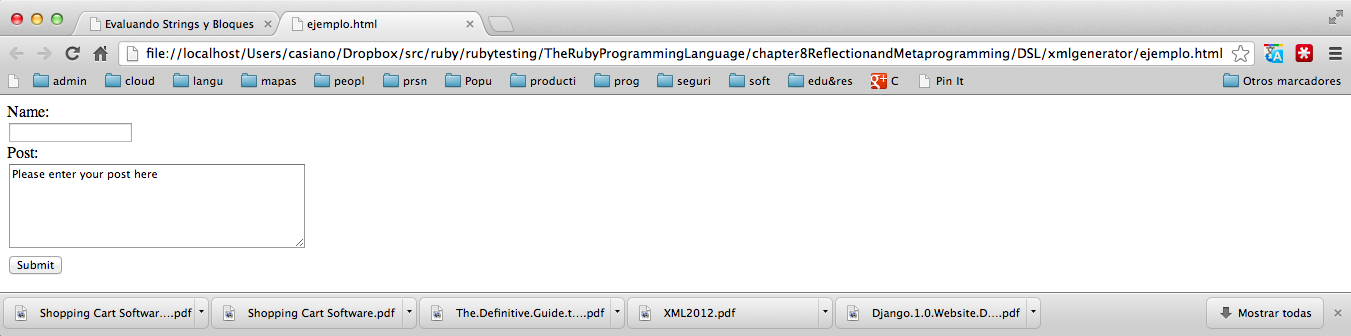
\includegraphics[scale=1]{chapter8/form.png}
\end{center}
\label{figure:formulario}
\caption{Formulario generado}
\end{figure}

\parrafo{Segundo DSL: Lenguaje para la Generación del DSL Anterior y su Validación}

Este DSL permite describir una gramática XML: que tags son permitidos
y para cada tag que atributos son legales y de que tipo son.
Se usaría así:

\begin{verbatim}
class HTMLForm < XMLGrammar
  element :form, :action => REQ,        # atributo requerido
                 :method => "GET",      # cadena: valor por defecto
                 :enctype => "application/x-www-form-urlencoded",
                 :name => OPT           # opcional
  element :input, :type => "text", :name => OPT, :value => OPT,
                  :maxlength => OPT, :size => OPT, :src => OPT,
                  :checked => BOOL, :disabled => BOOL, :readonly => BOOL
  element :textarea, :rows => REQ, :cols => REQ, :name => OPT,
                     :disabled => BOOL, :readonly => BOOL
  element :button, :name => OPT, :value => OPT,
                   :type => "submit", :disabled => OPT
  element :br
end
\end{verbatim}

El método \verb|element| construye un método de instancia 
con el nombre especificado (por ejemplo, \verb|:form|) como primer
argumento en la subclase (\verb|HTMLForm| en el ejemplo).
Como segundo argumento opcional recibe un hash especificando los atributos 
legales del elemento y de que tipo son (\verb|REQ| por requerido, \verb|OPT| por opcional,
una \String{} como en \verb|:method => "GET"| indica valor por defecto y \verb|BOOL| para atributos
cuyo valor es su propio nombre.

En el código anterior se crean métodos \verb|form|, \verb|input|, \verb|texarea|, \verb|button|
y \verb|br| en la clase \verb|HTMLForm|.



\parrafo{La Clase {\tt XMLGrammar}}


  \begin{latexonly}
    \begin{lstlisting}

class XMLGrammar
  # Create an instance of this class, specifying a stream or object to
  # hold the output. This can be any object that responds to <<(String).
  def initialize(out)
    @out = out  # Remember where to send our output
  end

  # Invoke the block in an instance that outputs to the specified stream.
  def self.generate(out, &block)
    new(out).instance_eval(&block)
  end

  # Define an allowed element (or tag) in the grammar.
  # This class method is the grammar-specification DSL
  # and defines the methods that constitute the XML-output DSL.
  def self.element(tagname, attributes={})
    @allowed_attributes ||= {}
    @allowed_attributes[tagname] = attributes

    class_eval %Q{
      def #{tagname}(attributes={}, &block)
        tag(:#{tagname},attributes,&block)
      end
    }
  end

  # These are constants used when defining attribute values.
  OPT = :opt     # for optional attributes
  REQ = :req     # for required attributes
  BOOL = :bool   # for attributes whose value is their own name

  def self.allowed_attributes
    @allowed_attributes
  end

  # Output the specified object as CDATA, return nil.
  def content(text)
    @out << text.to_s
    nil
  end

  # Output the specified object as a comment, return nil.
  def comment(text)
    @out << "<!-- #{text} -->\n"
    nil
  end

  # Output a tag with the specified name and attribute.
  # If there is a block, invoke it to output or return content.
  # Return nil.
  def tag(tagname, attributes={})
    # Output the tag name
    @out << "<#{tagname}"

    # Get the allowed attributes for this tag.
    allowed = self.class.allowed_attributes[tagname]

    # First, make sure that each of the attributes is allowed.
    # Assuming they are allowed, output all of the specified ones.
    attributes.each_pair do |key,value|
      raise "unknown attribute: #{key}" unless allowed.include?(key)
      @out << " #{key}='#{value}'"
    end

    # Now look through the allowed attributes, checking for 
    # required attributes that were omitted and for attributes with
    # default values that we can output.
    allowed.each_pair do |key,value|
      # If this attribute was already output, do nothing.
      next if attributes.has_key? key
      if (value == REQ)
        raise "required attribute '#{key}' missing in <#{tagname}>"
      elsif value.is_a? String
        @out << " #{key}='#{value}'"
      end
    end

    if block_given?
      # This block has content
      @out << '>'             # End the opening tag
      content = yield         # Invoke the block to output or return content
      if content              # If any content returned
        @out << content.to_s  # Output it as a string
      end
      @out << "</#{tagname}>\n" # Close the tag
    else 
      # Otherwise, this is an empty tag, so just close it.
      @out << "/>\n"
    end
    nil # Tags output themselves, so they don't return any content.
  end
end

    \end{lstlisting}
  \end{latexonly}
    \begin{rawhtml}
    <pre>
<span class="k">class</span> <span class="nc">XMLGrammar</span>
  <span class="c1"># Create an instance of this class, specifying a stream or object to</span>
  <span class="c1"># hold the output. This can be any object that responds to &lt;&lt;(String).</span>
  <span class="k">def</span> <span class="nf">initialize</span><span class="p">(</span><span class="n">out</span><span class="p">)</span>
    <span class="vi">@out</span> <span class="o">=</span> <span class="n">out</span>  <span class="c1"># Remember where to send our output</span>
  <span class="k">end</span>

  <span class="c1"># Invoke the block in an instance that outputs to the specified stream.</span>
  <span class="k">def</span> <span class="nc">self</span><span class="o">.</span><span class="nf">generate</span><span class="p">(</span><span class="n">out</span><span class="p">,</span> <span class="o">&amp;</span><span class="n">block</span><span class="p">)</span>
    <span class="kp">new</span><span class="p">(</span><span class="n">out</span><span class="p">)</span><span class="o">.</span><span class="n">instance_eval</span><span class="p">(</span><span class="o">&amp;</span><span class="n">block</span><span class="p">)</span>
  <span class="k">end</span>

  <span class="c1"># Define an allowed element (or tag) in the grammar.</span>
  <span class="c1"># This class method is the grammar-specification DSL</span>
  <span class="c1"># and defines the methods that constitute the XML-output DSL.</span>
  <span class="k">def</span> <span class="nc">self</span><span class="o">.</span><span class="nf">element</span><span class="p">(</span><span class="n">tagname</span><span class="p">,</span> <span class="n">attributes</span><span class="o">=</span><span class="p">{})</span>
    <span class="vi">@allowed_attributes</span> <span class="o">||=</span> <span class="p">{}</span>
    <span class="vi">@allowed_attributes</span><span class="o">[</span><span class="n">tagname</span><span class="o">]</span> <span class="o">=</span> <span class="n">attributes</span>

    <span class="nb">class_eval</span> <span class="sx">%Q{</span>
<span class="sx">      def </span><span class="si">#{</span><span class="n">tagname</span><span class="si">}</span><span class="sx">(attributes={}, &amp;block)</span>
<span class="sx">        tag(:</span><span class="si">#{</span><span class="n">tagname</span><span class="si">}</span><span class="sx">,attributes,&amp;block)</span>
<span class="sx">      end</span>
<span class="sx">    }</span>
  <span class="k">end</span>

  <span class="c1"># These are constants used when defining attribute values.</span>
  <span class="no">OPT</span> <span class="o">=</span> <span class="ss">:opt</span>     <span class="c1"># for optional attributes</span>
  <span class="no">REQ</span> <span class="o">=</span> <span class="ss">:req</span>     <span class="c1"># for required attributes</span>
  <span class="no">BOOL</span> <span class="o">=</span> <span class="ss">:bool</span>   <span class="c1"># for attributes whose value is their own name</span>

  <span class="k">def</span> <span class="nc">self</span><span class="o">.</span><span class="nf">allowed_attributes</span>
    <span class="vi">@allowed_attributes</span>
  <span class="k">end</span>

  <span class="c1"># Output the specified object as CDATA, return nil.</span>
  <span class="k">def</span> <span class="nf">content</span><span class="p">(</span><span class="n">text</span><span class="p">)</span>
    <span class="vi">@out</span> <span class="o">&lt;&lt;</span> <span class="n">text</span><span class="o">.</span><span class="n">to_s</span>
    <span class="kp">nil</span>
  <span class="k">end</span>

  <span class="c1"># Output the specified object as a comment, return nil.</span>
  <span class="k">def</span> <span class="nf">comment</span><span class="p">(</span><span class="n">text</span><span class="p">)</span>
    <span class="vi">@out</span> <span class="o">&lt;&lt;</span> <span class="s2">&quot;&lt;!-- </span><span class="si">#{</span><span class="n">text</span><span class="si">}</span><span class="s2"> --&gt;</span><span class="se">\n</span><span class="s2">&quot;</span>
    <span class="kp">nil</span>
  <span class="k">end</span>

  <span class="c1"># Output a tag with the specified name and attribute.</span>
  <span class="c1"># If there is a block, invoke it to output or return content.</span>
  <span class="c1"># Return nil.</span>
  <span class="k">def</span> <span class="nf">tag</span><span class="p">(</span><span class="n">tagname</span><span class="p">,</span> <span class="n">attributes</span><span class="o">=</span><span class="p">{})</span>
    <span class="c1"># Output the tag name</span>
    <span class="vi">@out</span> <span class="o">&lt;&lt;</span> <span class="s2">&quot;&lt;</span><span class="si">#{</span><span class="n">tagname</span><span class="si">}</span><span class="s2">&quot;</span>

    <span class="c1"># Get the allowed attributes for this tag.</span>
    <span class="n">allowed</span> <span class="o">=</span> <span class="nb">self</span><span class="o">.</span><span class="n">class</span><span class="o">.</span><span class="n">allowed_attributes</span><span class="o">[</span><span class="n">tagname</span><span class="o">]</span>

    <span class="c1"># First, make sure that each of the attributes is allowed.</span>
    <span class="c1"># Assuming they are allowed, output all of the specified ones.</span>
    <span class="n">attributes</span><span class="o">.</span><span class="n">each_pair</span> <span class="k">do</span> <span class="o">|</span><span class="n">key</span><span class="p">,</span><span class="n">value</span><span class="o">|</span>
      <span class="k">raise</span> <span class="s2">&quot;unknown attribute: </span><span class="si">#{</span><span class="n">key</span><span class="si">}</span><span class="s2">&quot;</span> <span class="k">unless</span> <span class="n">allowed</span><span class="o">.</span><span class="n">include?</span><span class="p">(</span><span class="n">key</span><span class="p">)</span>
      <span class="vi">@out</span> <span class="o">&lt;&lt;</span> <span class="s2">&quot; </span><span class="si">#{</span><span class="n">key</span><span class="si">}</span><span class="s2">=&#39;</span><span class="si">#{</span><span class="n">value</span><span class="si">}</span><span class="s2">&#39;&quot;</span>
    <span class="k">end</span>

    <span class="c1"># Now look through the allowed attributes, checking for </span>
    <span class="c1"># required attributes that were omitted and for attributes with</span>
    <span class="c1"># default values that we can output.</span>
    <span class="n">allowed</span><span class="o">.</span><span class="n">each_pair</span> <span class="k">do</span> <span class="o">|</span><span class="n">key</span><span class="p">,</span><span class="n">value</span><span class="o">|</span>
      <span class="c1"># If this attribute was already output, do nothing.</span>
      <span class="k">next</span> <span class="k">if</span> <span class="n">attributes</span><span class="o">.</span><span class="n">has_key?</span> <span class="n">key</span>
      <span class="k">if</span> <span class="p">(</span><span class="n">value</span> <span class="o">==</span> <span class="no">REQ</span><span class="p">)</span>
        <span class="k">raise</span> <span class="s2">&quot;required attribute &#39;</span><span class="si">#{</span><span class="n">key</span><span class="si">}</span><span class="s2">&#39; missing in &lt;</span><span class="si">#{</span><span class="n">tagname</span><span class="si">}</span><span class="s2">&gt;&quot;</span>
      <span class="k">elsif</span> <span class="n">value</span><span class="o">.</span><span class="n">is_a?</span> <span class="nb">String</span>
        <span class="vi">@out</span> <span class="o">&lt;&lt;</span> <span class="s2">&quot; </span><span class="si">#{</span><span class="n">key</span><span class="si">}</span><span class="s2">=&#39;</span><span class="si">#{</span><span class="n">value</span><span class="si">}</span><span class="s2">&#39;&quot;</span>
      <span class="k">end</span>
    <span class="k">end</span>

    <span class="k">if</span> <span class="nb">block_given?</span>
      <span class="c1"># This block has content</span>
      <span class="vi">@out</span> <span class="o">&lt;&lt;</span> <span class="s1">&#39;&gt;&#39;</span>             <span class="c1"># End the opening tag</span>
      <span class="n">content</span> <span class="o">=</span> <span class="k">yield</span>         <span class="c1"># Invoke the block to output or return content</span>
      <span class="k">if</span> <span class="n">content</span>              <span class="c1"># If any content returned</span>
        <span class="vi">@out</span> <span class="o">&lt;&lt;</span> <span class="n">content</span><span class="o">.</span><span class="n">to_s</span>  <span class="c1"># Output it as a string</span>
      <span class="k">end</span>
      <span class="vi">@out</span> <span class="o">&lt;&lt;</span> <span class="s2">&quot;&lt;/</span><span class="si">#{</span><span class="n">tagname</span><span class="si">}</span><span class="s2">&gt;</span><span class="se">\n</span><span class="s2">&quot;</span> <span class="c1"># Close the tag</span>
    <span class="k">else</span> 
      <span class="c1"># Otherwise, this is an empty tag, so just close it.</span>
      <span class="vi">@out</span> <span class="o">&lt;&lt;</span> <span class="s2">&quot;/&gt;</span><span class="se">\n</span><span class="s2">&quot;</span>
    <span class="k">end</span>
    <span class="kp">nil</span> <span class="c1"># Tags output themselves, so they don&#39;t return any content.</span>
  <span class="k">end</span>
<span class="k">end</span>
    </pre>
    \end{rawhtml}
  

\parrafo{Código Completo}


  \begin{latexonly}
    \begin{lstlisting}

class XMLGrammar
  # Create an instance of this class, specifying a stream or object to
  # hold the output. This can be any object that responds to <<(String).
  def initialize(out)
    @out = out  # Remember where to send our output
  end

  # Invoke the block in an instance that outputs to the specified stream.
  def self.generate(out, &block)
    new(out).instance_eval(&block)
  end

  # Define an allowed element (or tag) in the grammar.
  # This class method is the grammar-specification DSL
  # and defines the methods that constitute the XML-output DSL.
  def self.element(tagname, attributes={})
    @allowed_attributes ||= {}
    @allowed_attributes[tagname] = attributes

    class_eval %Q{
      def #{tagname}(attributes={}, &block)
        tag(:#{tagname},attributes,&block)
      end
    }
  end

  # These are constants used when defining attribute values.
  OPT = :opt     # for optional attributes
  REQ = :req     # for required attributes
  BOOL = :bool   # for attributes whose value is their own name

  def self.allowed_attributes
    @allowed_attributes
  end

  # Output the specified object as CDATA, return nil.
  def content(text)
    @out << text.to_s
    nil
  end

  # Output the specified object as a comment, return nil.
  def comment(text)
    @out << "<!-- #{text} -->\n"
    nil
  end

  # Output a tag with the specified name and attribute.
  # If there is a block, invoke it to output or return content.
  # Return nil.
  def tag(tagname, attributes={})
    # Output the tag name
    @out << "<#{tagname}"

    # Get the allowed attributes for this tag.
    allowed = self.class.allowed_attributes[tagname]

    # First, make sure that each of the attributes is allowed.
    # Assuming they are allowed, output all of the specified ones.
    attributes.each_pair do |key,value|
      raise "unknown attribute: #{key}" unless allowed.include?(key)
      @out << " #{key}='#{value}'"
    end

    # Now look through the allowed attributes, checking for 
    # required attributes that were omitted and for attributes with
    # default values that we can output.
    allowed.each_pair do |key,value|
      # If this attribute was already output, do nothing.
      next if attributes.has_key? key
      if (value == REQ)
        raise "required attribute '#{key}' missing in <#{tagname}>"
      elsif value.is_a? String
        @out << " #{key}='#{value}'"
      end
    end

    if block_given?
      # This block has content
      @out << '>'             # End the opening tag
      content = yield         # Invoke the block to output or return content
      if content              # If any content returned
        @out << content.to_s  # Output it as a string
      end
      @out << "</#{tagname}>\n" # Close the tag
    else 
      # Otherwise, this is an empty tag, so just close it.
      @out << "/>\n"
    end
    nil # Tags output themselves, so they don't return any content.
  end
end

class HTMLForm < XMLGrammar
  element :form, :action => REQ,
                 :method => "GET",
                 :enctype => "application/x-www-form-urlencoded",
                 :name => OPT
  element :input, :type => "text", :name => OPT, :value => OPT,
                  :maxlength => OPT, :size => OPT, :src => OPT,
                  :checked => BOOL, :disabled => BOOL, :readonly => BOOL
  element :textarea, :rows => REQ, :cols => REQ, :name => OPT,
                     :disabled => BOOL, :readonly => BOOL
  element :button, :name => OPT, :value => OPT,
                   :type => "submit", :disabled => OPT
  element :br
end

HTMLForm.generate(STDOUT) do
  comment "This is a simple HTML form"
  form :name => "registration",
       :action => "http://www.example.com/register.cgi" do
    content "Name:"
    br
    input :name => "name"
    br
    content "Post:"
    br
    textarea :name => "address", :rows=>6, :cols=>40 do
      "Please enter your post here"
    end
    br
    button { "Submit" }
  end
end

    \end{lstlisting}
  \end{latexonly}
    \begin{rawhtml}
    <pre>
<span class="k">class</span> <span class="nc">XMLGrammar</span>
  <span class="c1"># Create an instance of this class, specifying a stream or object to</span>
  <span class="c1"># hold the output. This can be any object that responds to &lt;&lt;(String).</span>
  <span class="k">def</span> <span class="nf">initialize</span><span class="p">(</span><span class="n">out</span><span class="p">)</span>
    <span class="vi">@out</span> <span class="o">=</span> <span class="n">out</span>  <span class="c1"># Remember where to send our output</span>
  <span class="k">end</span>

  <span class="c1"># Invoke the block in an instance that outputs to the specified stream.</span>
  <span class="k">def</span> <span class="nc">self</span><span class="o">.</span><span class="nf">generate</span><span class="p">(</span><span class="n">out</span><span class="p">,</span> <span class="o">&amp;</span><span class="n">block</span><span class="p">)</span>
    <span class="kp">new</span><span class="p">(</span><span class="n">out</span><span class="p">)</span><span class="o">.</span><span class="n">instance_eval</span><span class="p">(</span><span class="o">&amp;</span><span class="n">block</span><span class="p">)</span>
  <span class="k">end</span>

  <span class="c1"># Define an allowed element (or tag) in the grammar.</span>
  <span class="c1"># This class method is the grammar-specification DSL</span>
  <span class="c1"># and defines the methods that constitute the XML-output DSL.</span>
  <span class="k">def</span> <span class="nc">self</span><span class="o">.</span><span class="nf">element</span><span class="p">(</span><span class="n">tagname</span><span class="p">,</span> <span class="n">attributes</span><span class="o">=</span><span class="p">{})</span>
    <span class="vi">@allowed_attributes</span> <span class="o">||=</span> <span class="p">{}</span>
    <span class="vi">@allowed_attributes</span><span class="o">[</span><span class="n">tagname</span><span class="o">]</span> <span class="o">=</span> <span class="n">attributes</span>

    <span class="nb">class_eval</span> <span class="sx">%Q{</span>
<span class="sx">      def </span><span class="si">#{</span><span class="n">tagname</span><span class="si">}</span><span class="sx">(attributes={}, &amp;block)</span>
<span class="sx">        tag(:</span><span class="si">#{</span><span class="n">tagname</span><span class="si">}</span><span class="sx">,attributes,&amp;block)</span>
<span class="sx">      end</span>
<span class="sx">    }</span>
  <span class="k">end</span>

  <span class="c1"># These are constants used when defining attribute values.</span>
  <span class="no">OPT</span> <span class="o">=</span> <span class="ss">:opt</span>     <span class="c1"># for optional attributes</span>
  <span class="no">REQ</span> <span class="o">=</span> <span class="ss">:req</span>     <span class="c1"># for required attributes</span>
  <span class="no">BOOL</span> <span class="o">=</span> <span class="ss">:bool</span>   <span class="c1"># for attributes whose value is their own name</span>

  <span class="k">def</span> <span class="nc">self</span><span class="o">.</span><span class="nf">allowed_attributes</span>
    <span class="vi">@allowed_attributes</span>
  <span class="k">end</span>

  <span class="c1"># Output the specified object as CDATA, return nil.</span>
  <span class="k">def</span> <span class="nf">content</span><span class="p">(</span><span class="n">text</span><span class="p">)</span>
    <span class="vi">@out</span> <span class="o">&lt;&lt;</span> <span class="n">text</span><span class="o">.</span><span class="n">to_s</span>
    <span class="kp">nil</span>
  <span class="k">end</span>

  <span class="c1"># Output the specified object as a comment, return nil.</span>
  <span class="k">def</span> <span class="nf">comment</span><span class="p">(</span><span class="n">text</span><span class="p">)</span>
    <span class="vi">@out</span> <span class="o">&lt;&lt;</span> <span class="s2">&quot;&lt;!-- </span><span class="si">#{</span><span class="n">text</span><span class="si">}</span><span class="s2"> --&gt;</span><span class="se">\n</span><span class="s2">&quot;</span>
    <span class="kp">nil</span>
  <span class="k">end</span>

  <span class="c1"># Output a tag with the specified name and attribute.</span>
  <span class="c1"># If there is a block, invoke it to output or return content.</span>
  <span class="c1"># Return nil.</span>
  <span class="k">def</span> <span class="nf">tag</span><span class="p">(</span><span class="n">tagname</span><span class="p">,</span> <span class="n">attributes</span><span class="o">=</span><span class="p">{})</span>
    <span class="c1"># Output the tag name</span>
    <span class="vi">@out</span> <span class="o">&lt;&lt;</span> <span class="s2">&quot;&lt;</span><span class="si">#{</span><span class="n">tagname</span><span class="si">}</span><span class="s2">&quot;</span>

    <span class="c1"># Get the allowed attributes for this tag.</span>
    <span class="n">allowed</span> <span class="o">=</span> <span class="nb">self</span><span class="o">.</span><span class="n">class</span><span class="o">.</span><span class="n">allowed_attributes</span><span class="o">[</span><span class="n">tagname</span><span class="o">]</span>

    <span class="c1"># First, make sure that each of the attributes is allowed.</span>
    <span class="c1"># Assuming they are allowed, output all of the specified ones.</span>
    <span class="n">attributes</span><span class="o">.</span><span class="n">each_pair</span> <span class="k">do</span> <span class="o">|</span><span class="n">key</span><span class="p">,</span><span class="n">value</span><span class="o">|</span>
      <span class="k">raise</span> <span class="s2">&quot;unknown attribute: </span><span class="si">#{</span><span class="n">key</span><span class="si">}</span><span class="s2">&quot;</span> <span class="k">unless</span> <span class="n">allowed</span><span class="o">.</span><span class="n">include?</span><span class="p">(</span><span class="n">key</span><span class="p">)</span>
      <span class="vi">@out</span> <span class="o">&lt;&lt;</span> <span class="s2">&quot; </span><span class="si">#{</span><span class="n">key</span><span class="si">}</span><span class="s2">=&#39;</span><span class="si">#{</span><span class="n">value</span><span class="si">}</span><span class="s2">&#39;&quot;</span>
    <span class="k">end</span>

    <span class="c1"># Now look through the allowed attributes, checking for </span>
    <span class="c1"># required attributes that were omitted and for attributes with</span>
    <span class="c1"># default values that we can output.</span>
    <span class="n">allowed</span><span class="o">.</span><span class="n">each_pair</span> <span class="k">do</span> <span class="o">|</span><span class="n">key</span><span class="p">,</span><span class="n">value</span><span class="o">|</span>
      <span class="c1"># If this attribute was already output, do nothing.</span>
      <span class="k">next</span> <span class="k">if</span> <span class="n">attributes</span><span class="o">.</span><span class="n">has_key?</span> <span class="n">key</span>
      <span class="k">if</span> <span class="p">(</span><span class="n">value</span> <span class="o">==</span> <span class="no">REQ</span><span class="p">)</span>
        <span class="k">raise</span> <span class="s2">&quot;required attribute &#39;</span><span class="si">#{</span><span class="n">key</span><span class="si">}</span><span class="s2">&#39; missing in &lt;</span><span class="si">#{</span><span class="n">tagname</span><span class="si">}</span><span class="s2">&gt;&quot;</span>
      <span class="k">elsif</span> <span class="n">value</span><span class="o">.</span><span class="n">is_a?</span> <span class="nb">String</span>
        <span class="vi">@out</span> <span class="o">&lt;&lt;</span> <span class="s2">&quot; </span><span class="si">#{</span><span class="n">key</span><span class="si">}</span><span class="s2">=&#39;</span><span class="si">#{</span><span class="n">value</span><span class="si">}</span><span class="s2">&#39;&quot;</span>
      <span class="k">end</span>
    <span class="k">end</span>

    <span class="k">if</span> <span class="nb">block_given?</span>
      <span class="c1"># This block has content</span>
      <span class="vi">@out</span> <span class="o">&lt;&lt;</span> <span class="s1">&#39;&gt;&#39;</span>             <span class="c1"># End the opening tag</span>
      <span class="n">content</span> <span class="o">=</span> <span class="k">yield</span>         <span class="c1"># Invoke the block to output or return content</span>
      <span class="k">if</span> <span class="n">content</span>              <span class="c1"># If any content returned</span>
        <span class="vi">@out</span> <span class="o">&lt;&lt;</span> <span class="n">content</span><span class="o">.</span><span class="n">to_s</span>  <span class="c1"># Output it as a string</span>
      <span class="k">end</span>
      <span class="vi">@out</span> <span class="o">&lt;&lt;</span> <span class="s2">&quot;&lt;/</span><span class="si">#{</span><span class="n">tagname</span><span class="si">}</span><span class="s2">&gt;</span><span class="se">\n</span><span class="s2">&quot;</span> <span class="c1"># Close the tag</span>
    <span class="k">else</span> 
      <span class="c1"># Otherwise, this is an empty tag, so just close it.</span>
      <span class="vi">@out</span> <span class="o">&lt;&lt;</span> <span class="s2">&quot;/&gt;</span><span class="se">\n</span><span class="s2">&quot;</span>
    <span class="k">end</span>
    <span class="kp">nil</span> <span class="c1"># Tags output themselves, so they don&#39;t return any content.</span>
  <span class="k">end</span>
<span class="k">end</span>

<span class="k">class</span> <span class="nc">HTMLForm</span> <span class="o">&lt;</span> <span class="no">XMLGrammar</span>
  <span class="n">element</span> <span class="ss">:form</span><span class="p">,</span> <span class="ss">:action</span> <span class="o">=&gt;</span> <span class="no">REQ</span><span class="p">,</span>
                 <span class="ss">:method</span> <span class="o">=&gt;</span> <span class="s2">&quot;GET&quot;</span><span class="p">,</span>
                 <span class="ss">:enctype</span> <span class="o">=&gt;</span> <span class="s2">&quot;application/x-www-form-urlencoded&quot;</span><span class="p">,</span>
                 <span class="ss">:name</span> <span class="o">=&gt;</span> <span class="no">OPT</span>
  <span class="n">element</span> <span class="ss">:input</span><span class="p">,</span> <span class="ss">:type</span> <span class="o">=&gt;</span> <span class="s2">&quot;text&quot;</span><span class="p">,</span> <span class="ss">:name</span> <span class="o">=&gt;</span> <span class="no">OPT</span><span class="p">,</span> <span class="ss">:value</span> <span class="o">=&gt;</span> <span class="no">OPT</span><span class="p">,</span>
                  <span class="ss">:maxlength</span> <span class="o">=&gt;</span> <span class="no">OPT</span><span class="p">,</span> <span class="ss">:size</span> <span class="o">=&gt;</span> <span class="no">OPT</span><span class="p">,</span> <span class="ss">:src</span> <span class="o">=&gt;</span> <span class="no">OPT</span><span class="p">,</span>
                  <span class="ss">:checked</span> <span class="o">=&gt;</span> <span class="no">BOOL</span><span class="p">,</span> <span class="ss">:disabled</span> <span class="o">=&gt;</span> <span class="no">BOOL</span><span class="p">,</span> <span class="ss">:readonly</span> <span class="o">=&gt;</span> <span class="no">BOOL</span>
  <span class="n">element</span> <span class="ss">:textarea</span><span class="p">,</span> <span class="ss">:rows</span> <span class="o">=&gt;</span> <span class="no">REQ</span><span class="p">,</span> <span class="ss">:cols</span> <span class="o">=&gt;</span> <span class="no">REQ</span><span class="p">,</span> <span class="ss">:name</span> <span class="o">=&gt;</span> <span class="no">OPT</span><span class="p">,</span>
                     <span class="ss">:disabled</span> <span class="o">=&gt;</span> <span class="no">BOOL</span><span class="p">,</span> <span class="ss">:readonly</span> <span class="o">=&gt;</span> <span class="no">BOOL</span>
  <span class="n">element</span> <span class="ss">:button</span><span class="p">,</span> <span class="ss">:name</span> <span class="o">=&gt;</span> <span class="no">OPT</span><span class="p">,</span> <span class="ss">:value</span> <span class="o">=&gt;</span> <span class="no">OPT</span><span class="p">,</span>
                   <span class="ss">:type</span> <span class="o">=&gt;</span> <span class="s2">&quot;submit&quot;</span><span class="p">,</span> <span class="ss">:disabled</span> <span class="o">=&gt;</span> <span class="no">OPT</span>
  <span class="n">element</span> <span class="ss">:br</span>
<span class="k">end</span>

<span class="no">HTMLForm</span><span class="o">.</span><span class="n">generate</span><span class="p">(</span><span class="no">STDOUT</span><span class="p">)</span> <span class="k">do</span>
  <span class="n">comment</span> <span class="s2">&quot;This is a simple HTML form&quot;</span>
  <span class="n">form</span> <span class="ss">:name</span> <span class="o">=&gt;</span> <span class="s2">&quot;registration&quot;</span><span class="p">,</span>
       <span class="ss">:action</span> <span class="o">=&gt;</span> <span class="s2">&quot;http://www.example.com/register.cgi&quot;</span> <span class="k">do</span>
    <span class="n">content</span> <span class="s2">&quot;Name:&quot;</span>
    <span class="n">br</span>
    <span class="n">input</span> <span class="ss">:name</span> <span class="o">=&gt;</span> <span class="s2">&quot;name&quot;</span>
    <span class="n">br</span>
    <span class="n">content</span> <span class="s2">&quot;Post:&quot;</span>
    <span class="n">br</span>
    <span class="n">textarea</span> <span class="ss">:name</span> <span class="o">=&gt;</span> <span class="s2">&quot;address&quot;</span><span class="p">,</span> <span class="ss">:rows</span><span class="o">=&gt;</span><span class="mi">6</span><span class="p">,</span> <span class="ss">:cols</span><span class="o">=&gt;</span><span class="mi">40</span> <span class="k">do</span>
      <span class="s2">&quot;Please enter your post here&quot;</span>
    <span class="k">end</span>
    <span class="n">br</span>
    <span class="n">button</span> <span class="p">{</span> <span class="s2">&quot;Submit&quot;</span> <span class="p">}</span>
  <span class="k">end</span>
<span class="k">end</span>
    </pre>
    \end{rawhtml}
  


\sectionpractica{DSL: Redacción de Cuestionarios I (Sin Contexto)}
\label{sectionpractica:DSL1}
Se trata de escribir un programa que redacte cuestionarios.
En principio, sólo soportaremos preguntas del tipo selección múltiple:

\begin{verbatim}
1. ¿En que año Cristobal Colón descubrió América?
      1 - 1942
      2 - 1492
      3 - 1808
      4 - 1914
Su respuesta:
\end{verbatim}
Debe definir una clase \verb|Quiz| que soporte un pequeño lenguaje
en el que las preguntas puedan ser especificadas.
El constructor de \verb|Quiz| va seguido de un bloque al que pasa
como argumento el objeto \verb|e| que representa al examen:

\begin{verbatim}
quiz = Quiz.new("Cuestionario de PFS 10/12/2011") do |e|
  e.question '¿En que año Cristobal Colón descubrió América?',
    e.wrong =>'1942',
    e.right =>'1492',
    e.wrong =>'1808',
    e.wrong =>'1914'
  
  a = rand(10)
  b = rand(10)
  e.question "#{a}+#{b} = ",
    e.wrong =>"44",
    e.wrong =>"#{a + b + 2}",
    e.right =>"#{a + b}",
    e.wrong =>"#{a + b - 2}"
end

quiz.run
\end{verbatim}
El programa anterior podría producir una salida parecida a esta:

\begin{verbatim}
MacBookdeCasiano:chapter8ReflectionandMetaprogramming casiano$ ruby Quiz.rb 
Cuestionario de PFS 10/12/2011

¿En que año Cristobal Colón descubrió América?

  1 -  1942
  2 -  1492
  3 -  1808
  4 -  1914

Su respuesta: 3
0+8 = 

  1 -  44
  2 -  10
  3 -  8
  4 -  6

Su respuesta: 1
0 respuestas correctas de un total de 2.
MacBookdeCasiano:chapter8ReflectionandMetaprogramming casiano$ 
\end{verbatim}

\begin{itemize}
\item Los cuestionarios deberían tener un método \verb|to_s| que devuelve una \String{}
conteniendo el examen en texto plano.
Así al imprimir el objeto \verb|quiz| del ejemplo anterior:
\begin{verbatim}
puts quiz
puts "************************"
\end{verbatim}
obtendríamos como salida:
\begin{verbatim}
Cuestionario de PFS 10/12/2011

¿En que año Cristobal Colón descubrió América?

  1 -  1942
  2 -  1492
  3 -  1808
  4 -  1914


0+8 = 

  1 -  44
  2 -  10
  3 -  8
  4 -  6


************************
\end{verbatim}
\item Los cuestionarios deberían tener un método \verb|run| que formulará
cada una de las preguntas del cuestionario y mostrara el porcentaje de aciertos
\item Puede que le interese crear tres clases, una para modelar las respuestas (\verb|Answer|),
otra para modelar las preguntas (\verb|Question|) y una tercera para el cuestionario (\verb|Quiz|)
\item  El método \verb|question| recibe dos argumentos. El primero es el título del examen, el segundo es un hash:
\begin{verbatim}
  e.question '¿En que año Cristobal Colón descubrió América?',
    e.wrong =>'1942',
    e.right =>'1492',
    e.wrong =>'1808',
    e.wrong =>'1914'
\end{verbatim}
de modo que la llamada, realmente es equivalente a:
\begin{verbatim}
  e.question('¿En que año Cristobal Colón descubrió América?',
    {e.wrong =>'1942', e.right =>'1492', e.wrong =>'1808', e.wrong =>'1914'})
\end{verbatim}
si el segundo argumento de \verb|question| es un hash y las claves son \verb|:wrong| y \verb|:right| se va a 
producir una colisión y el último valor sobreescribirá a los anteriores. ¿Como resolverlo?
Una posible forma de hacerlo es que los métodos \verb|wrong| y \verb|right| diferencien las ocurrencias de las repsuestas
usando un contador \verb|@counter|:
\begin{verbatim}
 def wrong
    @counter += 1
    [@counter, WRONG]
  end
\end{verbatim}
\item Escriba un método \verb|to_html| que genere una página describiendo el examen. Use \ERB{}. 
\item
Opcionalmente
puede incluir hojas de estilo, javascript, etc. en el HTML generado
\item Use TDD con \rspec{}
\item Use Unit Testing
\item Use Continuous Integration (Travis)
\item Use Continuous Testing (Guard)
\item Documente su gema (véase
\htmladdnormallink{\cei{RDOC::Markup}}{http://docs.seattlerb.org/rdoc/RDoc/Markup.html}
o
\htmladdnormallink{\cei{RDOC}}{http://rdoc.sourceforge.net/doc/index.html} 
o 
\htmladdnormallink{\cei{YARD}}{http://yardoc.org}). 
\item Cree una gema \verb|ull-etsii-aluXX-quiz|
\item Publique la gema en \rubygems{}
\item Indique la URL de su repositorio en \github{} y la URL en \rubygems{}
\end{itemize}



\sectionpractica{DSL: Redacción de Cuestionarios II (Con Contexto)}
\label{sectionpractica:DSL}
Se trata de escribir un programa que redacte cuestionarios.
En principio, sólo soportaremos preguntas del tipo selección múltiple:

\begin{verbatim}
1. ¿En que año Cristobal Colón descubrió América?
      1 - 1942
      2 - 1492
      3 - 1808
      4 - 1914
Su respuesta:
\end{verbatim}
Debe definir una API que soporte un pequeño lenguaje
en el que las preguntas puedan ser especificadas de una forma natural.
algo así vale:

\begin{verbatim}
quiz = Quiz.new("Cuestionario de PFS 10/12/2011") {
  question '¿En que año Cristobal Colón descubrió América?',
    wrong =>'1942',
    right =>'1492',
    wrong =>'1808',
    wrong =>'1914'
  
  a = rand(10)
  b = rand(10)
  question "#{a}+#{b} = ",
    wrong =>"44",
    wrong =>"#{a + b + 2}",
    right =>"#{a + b}",
    wrong =>"#{a + b - 2}"
}

puts quiz
puts "************************"
quiz.run
\end{verbatim}
El programa anterior podría producir una salida parecida a esta:

\begin{verbatim}
MacBookdeCasiano:chapter8ReflectionandMetaprogramming casiano$ ruby Quiz.rb 
Cuestionario de PFS 10/12/2011

¿En que año Cristobal Colón descubrió América?

  1 -  1942
  2 -  1492
  3 -  1808
  4 -  1914


0+8 = 

  1 -  44
  2 -  10
  3 -  8
  4 -  6


************************
Cuestionario de PFS 10/12/2011

¿En que año Cristobal Colón descubrió América?

  1 -  1942
  2 -  1492
  3 -  1808
  4 -  1914

Su respuesta: 3
0+8 = 

  1 -  44
  2 -  10
  3 -  8
  4 -  6

Su respuesta: 1
0 respuestas correctas de un total de 2.
MacBookdeCasiano:chapter8ReflectionandMetaprogramming casiano$ 
\end{verbatim}

\begin{itemize}
\item Los cuestionarios deberían tener un método \verb|to_s|
\item Los cuestionarios deberían tener un método \verb|run| que formulara
cada una de las preguntas del cuestionario y mostrara el porcentaje de aciertos
\item Puede que le interese crear tres clases, una para las respuestas (\verb|Answer|),
otra para las preguntas (\verb|Question|) y una para el cuestionario (\verb|Quiz|)
\item  Hay un problema con la llamada al método \verb|question|:
\begin{verbatim}
  question '¿En que año Cristobal Colón descubrió América?',
    wrong =>'1942',
    right =>'1492',
    wrong =>'1808',
    wrong =>'1914'
\end{verbatim}
si el segundo argumento es un hash y las claves son \verb|wrong| y \verb|right| se va a 
producir una colisión y el último valor sobreescribirá a los anteriores. ¿Se puede resolver?
\end{itemize}


\sectionpractica{HTML DSL}
\label{sectionpractica:htmldsl}
En esta práctica deberá escribir una clase que provea una funcionalidad 
parecida (por supuesto, no completa)
 a la de la librería
\htmladdnormallink{markaby}{http://markaby.rubyforge.org/}.
La librería provee métodos \verb|html|, \verb|body|, \verb|h1|, etc. que permiten 
la escritura de los correspondientes tags HTML:
\begin{verbatim}
 require 'markaby'

  mab = Markaby::Builder.new
  mab.html do
    head { title "Boats.com" }
    body do
      h1 "Boats.com has great deals"
      ul do
        li "$49 for a canoe"
        li "$39 for a raft"
        li "$29 for a huge boot that floats and can fit 5 people"
      end
    end
  end
  puts mab.to_s
\end{verbatim}
Los métodos, como \verb|b| reciben como primer argumento una cadena que es la que hay que rodear entre
las marcas \verb|<b>| y \verb|</b>|.
También pueden recibir opcionalmente un segundo argumento que sea un hash
especificando los atributos asociados con el tag:
\begin{verbatim}
a "google", :href => "http://www.google.com", :name => "foo"
\end{verbatim}
que debería dar lugar a un texto parecido a este:
\begin{verbatim}
<a href = "http://www.google.com", name = "foo">google</a>
\end{verbatim}
Si en la llamada no se provee la cadena inicial, se deberá proveer un bloque.
Dicho bloque construye la cadena que se interpolará entre las marcas.
Así:
\begin{verbatim}
head { title "My wonderful home page" }
\end{verbatim}

debería producir la cadena:
\begin{verbatim}
<head><title>My wonderful home page</title></head>
\end{verbatim}
La ejecución de este código
\begin{verbatim}
~/chapter8ReflectionandMetaprogramming$ cat -n html.rb 
     1  class HTML
     2    attr_accessor :page
     3  
     4    def initialize........
     5      ....................
     6      ....................
     7    end
     8  
     9    def build_attr(attributes)
    10        ...........................................................
    11        ............................................................ 
    12    end
    13  
    14    def ..............(tag, *args)
    15      ...............................................
    16      ...............................................
    17      ...............................................
    18      ...............................................
    19      ...............................................
    20      ...............................................
    21      ...............................................
    22      ...............................................
    23      ...............................................
    24      ...............................................
    25      ...............................................
    26      ...............................................
    27    end
    28  
    29    def to_s
    30      ..............................................
    31    end
    32  end
    33  
    34  if __FILE__ == $0
    35    q= HTML.new {  
    36      html {
    37        head(:dir => "chazam", :lang => "spanish") { title "My wonderful home page" }
    38        body do
    39          h1 "Welcome to my home page!", :class => "chuchu", :lang => "spanish"
    40          b "My hobbies:"
    41          ul do
    42            li "Juggling"
    43            li "Knitting"
    44            li "Metaprogramming"
    45          end #ul
    46        end # body
    47      }
    48    }
    49    puts q
    50  end
\end{verbatim}
debería producir una salida parecida a esta:
\begin{verbatim}
~/chapter8ReflectionandMetaprogramming$ ruby html.rb 
<html>
<head dir = "chazam" lang = "spanish">
<title>
My wonderful home page
</title>
</head>
<body>
<h1 class = "chuchu" lang = "spanish">
Welcome to my home page!
</h1> <b>
My hobbies:
</b> <ul>
<li>
Juggling
</li> <li>
Knitting
</li> <li>
Metaprogramming
</li>
</ul>
</body>
</html>
\end{verbatim}

Repase las secciones 
\ref{seubsection:methodmissing}
y
\ref{subsection:instanceeval}.

\sectionpractica{HTML DSL con Git y Rake}
\label{sectionpracica:gitandrake}
Complete la práctica descrita en la sección
\ref{sectionpractica:htmldsl} con los siguientes requisitos:
\begin{itemize}
\item Use \verb|git| y \verb|github| para el desarrollo de la práctica. Creee 
en el repositorio un subproyecto LPP
y en el mismo un subproyecto para la práctica.
\item Documente el código
\item En el directorio \verb|lib| residirá la librería
\item Cree un directorio \verb|test| en el que residirán las pruebas
\item Escriba las pruebas. Recuerde:
  \begin{itemize}
  \item
  Todas las pruebas deben automatizarse
  \item
  Todos los fallos que se detecten deberían quedar traducidos en pruebas
  \item
  La aplicación debería pasar todas las pruebas después de cualquier modificación
  importante y también al final del día
  \item
  El desarrollo de las pruebas debería preceder el desarrollo 
  del código
  \item
  Todos los requerimientos deben ser expresados en forma de pruebas
  \item
  El tiempo invertido en \emph{Comprobar} (\emph{testing}) y el
  tiempo invertido en \emph{Depurar} (\emph{debugging})
  mantiene una relación inversa.  \emph{Cuanto menor es el tiempo invertido
  en la preparación de pruebas mayor será nuestro tiempo de depuración}.
  Cuanto mejor sea nuestra suite de pruebas menor será el tiempo que necesitemos
  para fijar errores en nuestros programas.
  \item
  Las pruebas no aseguran la corrección de nuestro programa.
  Las pruebas descubren errores. Una prueba tiene éxito cuando falla y
  demuestra la presencia de un error.
  \item
  En palabras de Bruce Eckel (\emph{Thinking in Java}):
  \begin{it}
  \begin{quote}
  You can write all the prose, or create
  all the diagrams you want, describing how a class should behave and what it looks
  like, but nothing is as real as a set of tests. The former
  is a wish list, but the tests are a contract
  that is enforced by the compiler and the running program.
  It's hard to imagine a more concrete description of a class than the tests
  \end{quote}
  \end{it}
  \item
  Cuando escriba las pruebas invierta su escala de valores:
  \emph{Alégrese cuando una prueba descubre un error}.
  Es peor que el error esté ahí y no sea descubierto.
  \item Que comprobar:
  \begin{itemize}
  \item
  Convertir cualquier fallo que encontremos en una prueba
  \item
  Comprobar el funcionamiento en mas de una plataforma
  \item
  Dar valores de entrada erróneos o en el límite. Por ejemplo:
  \begin{itemize}
  \item
  Los valores máximo y mínimo posibles
  \item
  Cadenas vacías
  \item
  Cadenas multilínea
  \item
  Entradas con caracteres de control, etc.
  \item
  Valores como \verb|'0'|, \verb|'0E0'|, listas vacías, hashes vacíos, etc.
  \item
  Llamar sin argumentos a una rutina que los espera y viceversa
  \item
  Llamar a una rutina con mas argumentos de los que espera
  \item
  Llamar a una rutina con los argumentos en orden incorrecto
  \end{itemize}
  \item
  Estudie las interacciones y dependencias
  entre recursos que se da por sentado que están (pero que a veces pueden
  no estar.  Por ejemplo, un fichero con cuya existencia se cuenta)
  \item
  Estudie la dependencia de versiones del software instalado
  \item
  Compruebe que toda subrutina se prueba al menos una vez.
  Prepare para cada subrutina importante al menos una prueba
  que cubra el caso promedio y otra que compruebe
  su funcionamiento en casos límite.
  \item
  Estudie la escalabilidad de la distribución con valores tendiendo
  al límite. Ficheros grandes, números grandes, etc.
  \end{itemize}


  \end{itemize}

\item Cree un \verb|Rakefile| con diferentes objetivos:
  \begin{itemize}
  \item \verb|test| para ejecutar las pruebas
  \item \verb|dist| para crear un \verb|tar.gz| con todos los ficheros
  \item \verb|zip| para crear un \verb|zip| con todos los ficheros
  \item \verb|clean| para borrar ficheros temporales
  \end{itemize}
\end{itemize}

\section{Repaso}
\begin{enumerate}
\item ¿Cuanto vale \verb|self| en las líneas 5-8 cuando \verb|my_attr_reader| es llamado desde la línea 14?
\begin{verbatim}
MacBookdeCasiano:chapter8ReflectionandMetaprogramming casiano$ cat -n myAccessors.rb 
     1  class Module
     2    def my_attr_reader(*syms)
     3      syms.each { |s|
     4        class_eval %{
     5                      def #{s} 
     6                        @#{s} 
     7                      end
     8                    }
     9      }
    10    end
    11  end
    12  
    13  class Chuchu
    14    my_attr_reader :a, :b
    15  
    16    def initialize(a,b)
    17      @a, @b = a, b
    18    end
    19  end
\end{verbatim}
\item Rellene las partes que faltan en el código de la clase \verb|Quiz| que implementa un DSL para la escritura de cuestionarios.
Comente el código.
\begin{verbatim}
class Quiz
  RIGHT = :right
  WRONG = :wrong

  attr_accessor :name, :_________ 

  def initialize(name, &block)
    self.name = name
    self.questions = __

    @counter = 0
    _____________ &block
  end

  def question(text, answers)
    q = Question.new(text, answers)
    questions << q 
    @_______ = _
  end


  def to_s
    out = <<"EOQUIZ"
#{self.name}

#{self.questions.____("\n")}
EOQUIZ
  end

  def wrong
    @counter += 1
    [_______________]
  end

  def right
    @counter+= 1
    [_______________]
  end

  def run
    counter=0
    puts self.name+"\n\n"
    self.questions.each { |q| counter += 1 if q.ask }
    puts "#{counter} respuestas correctas de un total de #{@_________.size}."
  end
end
\end{verbatim}
\item Rellene las partes que faltan en el código de la clase \verb|Question| 
que implementa los objetos \verb|question| para
el DSL visto en clase para la escritura de cuestionarios. 
Comente el código.
\begin{verbatim}
class Question
  ORDER = 0
  KIND = 1
  attr_accessor :text, :answers

  def initialize(text, answers)
    @text = text
    @answers = answers.map { |k, v| _________________________________ }.sort
  end

  def to_s
    output = <<"EORECIPE"
#{_____}

#{
    out = ""
    @answers.each do |answer|
      out << "  #{answer}\n"
    end
    ___
}
EORECIPE
  end

  def ask
    begin
      puts self
      print "Su respuesta: " 
      answerno = gets.to_i - 1
    end while (answerno < 0 or answerno >= @_______.______)
    @answers[________].is_right? 
  end

end
\end{verbatim}
\item Rellene las partes que faltan en el código de la clase \verb|Answer| que implementa las respuestas
en el DSL para la escritura de cuestionarios.
Comente el código.
\begin{verbatim}
class Answer
  attr_accessor :____, :_____, :______

  def initialize(order, kind, answer)
    @kind, @order, @answer = kind, order, answer
  end

  def to_s
    "#{@order} -  #{answer}"
  end

  def is_right?
    ____________________
  end

  def ___(other)
    __________________________
  end

end
\end{verbatim}
\item
Complete las partes que faltan en el siguiente código que implementa el método
\verb|prun| de la práctica {\it Procesos Concurrentes}.
Comente el programa.
\begin{verbatim}
#!/usr/___/env ____ -w

def deb(m) 
  puts "#{$$}: #{m}" if $DEBUG
end


def getResult(chan)
  Marshal.____(chan.____)
end
  
def prun(p)
  pid, name, read = {}, {}, {}
  p.each { |n, code|
    read[n], write = IO.____

    pid[n] = fork do
      read[n]._____

      res = _________(n)

      write.syswrite ____________(res)

    end # fork

    write._____
  }

  name = pid.invert
  
  result = {}
  p.length.times { 
    i, s = Process._____ 
    n = _______

    result[n] = getResult(read[n])
    deb "Finished process '____' pid=____ with status #{s} result = ____________"
  }
  ______
end

res = prun(
     :one     => lambda { |n| "#{n} is 1" },
     :three   => lambda { |n| "#{n} is 3" },
     'two'    => lambda { |n| n*4 }
)
\end{verbatim}
\item
Complete las partes que faltan en el siguiente código 
de la práctica {\it Ordenar por Calificaciones}
que implementa la ordenación de un ficheros
de notas 
con el formato:
\begin{verbatim}
Ferrer Pérez, Eduardo & 9'6\\
\end{verbatim}
Se ordenan en orden decreciente de calificaciones.
Comente el programa.
\begin{verbatim}
~/rubytesting$ cat -n calif.rb 
     1  f = File.open('notas')
     2  x = f._________
     3  
     4  y = x.map { |alu| alu =~ /_____________________/;  ________ }
     5  h =  ____[__________]
     6  h.keys.each { |alu| h[alu].gsub!(/__________)/, '_____'); h[alu] = h[alu].____ }
     7  
     8  s = h.sort { |a,b| ____ <=> ____ }
     9  s.each { |x| puts "_________________________" }
\end{verbatim}

\item
Complete las partes que faltan en el siguiente código 
de la práctica {\it  La Calculadora}
que implementa una calculadora extensible 
de expresiones en postfijo
que admiten variables y asignación.
Comente el programa. %postfixwithhashfunctions3.rb
\begin{verbatim}
 1  class PostfixCalc
 2  
 3    attr_reader :stack
 4    attr_accessor :st
 5  
 6    def initialize(f) 
 7      @f = {
 8        '+' => lambda { |a,b| a+b },
 9        '*' => lambda { |a,b| a*b },
10        '-' => lambda { |a,b| a-b },
11        '/' => lambda { |a,b| a/b },
12        'p' => lambda { _____________ },
13        '!' => lambda { __________ },
14        '=' => lambda { _____________________ },
15      }
16      @f._____!(f)
17      @st = ________
18      @stack = __
19    end
20  
21   def eval(expr)
22      expr.gsub!(/____________________/, '\1 \2') # Se admite a= y b!
23      expr.split(/___/).each do |x|
24        case x
25          when *@f.keys
26            f = _____
27            ops = @stack.pop _______
28            b = f.call(_____)
29            @stack.push __ if __
30          when /^-?\d+(\.\d+)?$/
31            @stack.push ______
32          when /^[a-zA-Z_]\w*$/
33            _____________
34          else
35            ___________________________________________________________________       
36        end
37      end # each
38    end
39  end
..  ...
\end{verbatim}

\item
Complete las partes que faltan en el siguiente fragmento de código 
que implementa la práctica {\it  Conjuntos}
usando arrays.
Comente el programa.
\begin{verbatim}
 1  class Set2 
 2  
 3    attr_accessor :sep
 4    attr_reader :a
 5    protected :a
 6  
 7    def initialize(a)
 8      @sep = ', '
 9      @a = a.uniq.____
10    end
11  
12    def to_s
13      _______(@sep)
14    end
15  
16    def length 
17      _________
18    end
19  
20    alias cardinal ______
21  
22    def +(o)
23      Set2.new(________)
24    end
25  
26    def ^(o) # interseccion
27      Set2.new(________)
28    end
29  
30    def -(o)
31      Set2.new(________)
32    end
33  
34    def include?(x)
35      _____________
36    end
37  
38    def <(s)
39      if @a.length < s.a.length 
40        return true if @a.all? { |m| ______________ }
42      end
43      return false
44    end
45  
54    def ==(s)
55      _________
56    end
57  
58    def <=(s)
59      _________________________
60    end
\end{verbatim}
\item ¿Cual es la diferencia entre \verb|dup| y \verb|clone|?
\item ¿Cómo se llama el método que nos permite declarar
un método de clase como privado? % private_class_method
\item
¿Que hace El método \htmladdnormallink{const\_set}{http://www.ruby-doc.org/core-1.8.7/Module.html\#method-i-const\_set}
de la clase \htmladdnormallink{Module}{http://www.ruby-doc.org/core-1.8.7/Module.html}?
\item ¿Que retorna el método \verb|fork|? ¿Que argumentos lleva?
\item  ¿Que retorna el método \verb|pipe|? ¿En que clase está?
\item ¿Que hace el método \verb|wait2|?
\item ¿Que hace el método \verb|exit!|?
\item ¿Que es un proceso zombi?
\item ¿Que diferencias hay entre \verb|syswrite| y \verb|puts|?
\item ¿Cómo funciona el método \verb|popen|? (véase por ejemplo \ref{subsection:YAML})
\begin{verbatim}
  popen(cmd_string, mode="r" ) {|io| block } => obj
\end{verbatim}
\item ¿Que es YAML? ¿Para que sirve? (véase por ejemplo \ref{subsection:YAML})
\item ¿Cual es el resultado?
\begin{verbatim}
>> ww ||= 8
=> 
>> ww ||= 9
=> 
\end{verbatim}
\item Complete el código que falta. La clase \verb|SerializableProc| implementa
bloques de código serializables (véase \ref{Marshalling Lambdas y Procs}):
\begin{verbatim}
class SerializableProc

   def initialize( block )
     @block = block
     @block.sub!(/^/,'lambda ') unless @block =~/^\s*(?:lambda|proc)/
     @func = eval "#{@block}"
   end


   def call(* args)
     __________(* args)
   end

   def arity
     @func.arity
   end

   def _____(limit)
     ______
   end

   def ____._____(s)
     ________(s)
   end
end
\end{verbatim}
\item ¿Cuales son las salidas?
\begin{verbatim}
>> def tutu(n,m, &b) b.call() end
=> nil
>> tutu 2, {:a =>1, :b =>2} { puts "hello" }


>> tutu(2,{:a =>1, :b =>2}) { puts "hello" }


\end{verbatim}
\item  ¿Que hace el método \verb|extend| cuando es llamado en un objeto?
¿Que argumentos recibe? ¿Cual es la salida de estas sentencias? (véase \ref{subsection:extend})
\begin{verbatim}
>> module Chuchu
>> def hello; "hello" end
>> end
=> nil
>> s = {}
=> {}
>> s.extend Chuchu
=> {}
>> s.hello
=> 
\end{verbatim}
\item ¿Cual es el peligro de usar \verb|eval| en un entorno distribuído?
\item
Comente el siguiente programa y explica su comportamiento:
\begin{verbatim}
    def multiplier(n)
      lambda do |*arr| 
                arr.collect { |i| i*n } 
             end
    end
    
    doubler = multiplier(2)
    puts doubler[1, 2, 3]
    
    eval("n = 3", doubler.binding)
    puts doubler.call(1, 2, 3)
    
    eval("n = 5", doubler)
    puts doubler.call(1, 2, 3)
\end{verbatim}
\item ¿Que diferencias hay entre \basicobjecti{instance\_eval}, \modulei{class\_eval} y \verb|eval|?
\item ¿Que es un DSL? ¿Que es un DSL interno o empotrado?

\end{enumerate}
Repase los ejercicios
\ref{ejercicios:schwartz},
\ref{ejercicios:procesos},
\ref{ejercicios:hashes},
y
\ref{ejercicios:lambda}.

\section{Repaso}

\begin{itemize}
\item ¿Cuál es la salida de este programa?
\begin{verbatim}
~/rubytesting$ cat -n closure1.rb 
     1  def greetings
     2    x = "Goodbye"
     3    yield 
     4  end
     5  
     6  x = "Hello"
     7  puts greetings { "#{x} world" }
\end{verbatim}
\item ¿Cuál es la salida de este programa?
\begin{verbatim}
~/rubytesting$ cat -n blocks1_8.rb 
     1  def chuchu
     2    yield 2
     3  end
     4  
     5  x = 1
     6  chuchu { |x| }
     7  puts x
~/rubytesting$ ruby -v
ruby 1.8.7 (2010-01-10 patchlevel 249) [universal-darwin10.0]
~/rubytesting$ ruby blocks1_8.rb 

\end{verbatim}
\item ¿Cuál es la salida de este programa?
\begin{verbatim}
~/rubytesting$ cat -n blocks1_8.rb 
     1  def chuchu
     2    yield 2
     3  end
     4  
     5  x = 1
     6  chuchu { |x| }
     7  puts x
~/rubytesting$ sudo rvm install 1.9.2
...
Install of ruby-1.9.2-p290 - #complete 
~/rubytesting$  
~/rubytesting$ rvm list

rvm rubies

   ruby-1.9.2-p290 [ x86_64 ]

~/rubytesting$ rvm ruby-1.9.2-p290
~/rubytesting$ ruby -v
ruby 1.9.2p290 (2011-07-09 revision 32553) [x86_64-darwin10.8.0]
~/rubytesting$ ruby blocks1_8.rb 

\end{verbatim}
\htmladdnormallink{RVM}{http://beginrescueend.com/} {\it is a command-line tool which allows you to easily install, manage, and work with multiple ruby environments from interpreters to sets of gems.}
\item Dado el programa:
\begin{verbatim}
~/rubytesting$ cat -n scopes.rb 
     1  v1 = 1                  
     2  
     3  class Tutu
     4    v2 = 2                
     5    puts "%2d"%(__LINE__.to_s)+' '+local_variables.inspect    
     6  
     7    def my_method
     8      v3 = 3
     9      puts "%2d"%__LINE__.to_s+' '+local_variables.inspect
    10    end
    11  
    12    puts "%2d"%__LINE__.to_s+' '+local_variables.inspect    
    13  end
    14  
    15  obj = Tutu.new
    16  obj.my_method        
    17  obj.my_method        
    18  puts "%2d"%__LINE__.to_s+' '+local_variables.inspect      
\end{verbatim}
¿Cuál es la salida de este programa?
\begin{verbatim}
~/rubytesting$ ruby scopes.rb 
 5 .....................
12 .....................
 9 .....................
 9 .....................
18 .....................
\end{verbatim}
\item Dado el programa:
\begin{verbatim}
~/rubytesting$ cat -n instance_scope.rb 
     1  @var = "hello"
     2  
     3  class Tutu
     4    puts "Inside Tutu: #{@var}"
     5  end
     6  
     7  puts @var
\end{verbatim}
¿Cual es la salida de esta ejecución?
\begin{verbatim}
~/rubytesting$ ruby -w instance_scope.rb 


\end{verbatim}

\item Dado el programa:
\begin{verbatim}
~/rubytesting$ cat -n scopes2.rb 
     1  v1 = 1                  
     2  
     3  Tutu = Class.new do
     4    v2 = 2                
     5    puts "%2d"%(__LINE__.to_s)+' '+local_variables.inspect    
     6  
     7    def my_method
     8      v3 = 3
     9      puts "%2d"%__LINE__.to_s+' '+local_variables.inspect
    10    end
    11  
    12    puts "%2d"%__LINE__.to_s+' '+local_variables.inspect    
    13  end
    14  
    15  obj = Tutu.new
    16  obj.my_method        
    17  obj.my_method        
    18  puts "%2d"%__LINE__.to_s+' '+local_variables.inspect      
\end{verbatim}
¿Cuál es la salida de este programa?
\begin{verbatim}
~/rubytesting$ ruby scopes2.rb 
 5 .....................
12 .....................
 9 .....................
 9 .....................
18 .....................
\end{verbatim}

\item Dado el programa:
\begin{verbatim}
~/rubytesting$ cat -n scopes3.rb 
     1  v1 = 1                  
     2  
     3  Tutu = Class.new do
     4    v2 = 2                
     5    puts "%2d"%(__LINE__.to_s)+' '+local_variables.inspect    
     6  
     7    define_method :my_method  do
     8      v3 = 3
     9      puts "%2d"%__LINE__.to_s+' '+local_variables.inspect
    10    end
    11  
    12    puts "%2d"%__LINE__.to_s+' '+local_variables.inspect    
    13  end
    14  
    15  obj = Tutu.new
    16  obj.my_method        
    17  obj.my_method        
    18  puts "%2d"%__LINE__.to_s+' '+local_variables.inspect      
\end{verbatim}
¿Cuál es la salida de este programa?
\begin{verbatim}
~/rubytesting$ ruby scopes3.rb 
 5 .....................
12 .....................
 9 .....................
 9 .....................
18 .....................
\end{verbatim}
\item ¿En que clases está definido \verb|define_method|?
\item ¿Que visibilidad tiene \verb|define_method|? (público, privado, protegido) 
\item ¿En que clase queda definida el método creado por \verb|define_method|?
\item ¿Es posible llamar a \verb|define_method| con un receptor explícito?
\begin{verbatim}
Tutu.define_method
\end{verbatim}
\item Dado el programa:
\begin{verbatim}
~/rubytesting$ cat -n shared_scope2.rb 
     1  def define_methods
     2    shared = 5
     3    
     4    Kernel.send :define_method, :counter do
     5      shared
     6    end
     7  
     8    Kernel.send :define_method, :inc do |x|
     9      shared += x
    10    end
    11  end
    12  
    13  define_methods
    14  
    15  puts counter     
    16  inc(4)
    17  puts counter      
\end{verbatim}
\begin{itemize}
\item
¿Cuál es la salida de este programa?
\item
¿Por que no puede llamarse a \verb|define_method| en vez de \verb|Kernel.send define_method|?
\item
¿Donde (en que clase/objeto) estamos incorporando los métodos \verb|counter| e \verb|inc|?
\item
¿A que objeto/clase  esta siendo envíado el mensaje \verb|counter| en la línea 15?
\end{itemize}
\item
¿Cuál es la salida?
\begin{verbatim}
MacBook-Air-de-casiano:rubytesting casiano$ cat -n define_method.rb 
     1  class A
     2    def fred
     3      puts "In Fred"
     4    end
     5    def create_method(name, &block)
     6      self.class.send(:define_method, name, &block)
     7    end
     8    define_method(:wilma) { puts "Charge it!" }
     9  end
    10  class B < A
    11    define_method(:barney, instance_method(:fred))
    12  end
    13  a = B.new
    14  a.barney
    15  a.wilma
    16  a.create_method(:betty) { p self }
    17  a.betty
\end{verbatim}
\verb|instance_method| es definido en \rubymod{Module}.
Retorna un {\it UnboundMethod}.
\end{itemize}

\section{Repaso}

\begin{enumerate}
\item %dieta. reto dropbox
Complete el siguiente programa Ruby que resuelve el reto Dropbox
conocido como "El Problema de la Dieta" (partes en subrayado):
\begin{verbatim}
 1  def solve(goal, values)
 2    x = values.____
 3  
 4    subsets = lambda do |k|
 5      return { _______ } if k < 0
 6      old_sums = subsets[___]
 7  
 8      new_sums = ___
 9  
10      old_sums.keys.each do |p|
11        c = p + ____
12        new_sums[c] = _________________ if c <= goal
13      end
14  
15      return old_sums._____(new_sums) 
16    end
17  
18    z = subsets[values.________][goal] || []
19    x.values_at(*z)
20  end
21  
22  rdropbox = {
23    'free-lunch'    =>  802,
..    .......................,
34    'playing-drums'    =>  -295
35  }.invert
36  
37  s = solve(0, rdropbox.keys)
38  puts s.inspect
39  puts rdropbox.values_at(*s).inspect
\end{verbatim}
\item
Escriba los nombres de los métodos para listar los nombres (como cadenas)
de 
\begin{itemize}
\item las variables globales que estén definidas (\verb|________________|) 
\item de las variables locales que estén actualmente definidas (\verb|_______________|)
\item de las variables de instancia de un objeto (\verb|__________________|)
\item de las variables de clase o módulo (\verb|_______________|)
\item y de las constantes de una clase o módulo (\verb|_________|)
\end{itemize}
¿Cuales son métodos de instancia? ¿Cuáles de clase?

\item
El código que sigue implementa un motor para las expresiones regulares.
Para simplificar las expresiones, se han definido algunos operadores.
Siguen algunos ejemplos de uso:
\begin{verbatim}
  e = 'c'.re - +('d'.re | 'r'.re)   # /c(d|r)+/
  s = 'crddf'
  remaining = e[s]                  # s =~ /c(d|r)+/
  puts "/c(d|r)+/ '#{s}' Matched. Remaining = '#{remaining}'" if remaining
                              # /c(d|r)+/ 'crddf' Matched. Remaining = 'f' 
  e = 'c'.re - ~('d'.re | 'r'.re)   # /c(d|r)*/
  s = 'cdrdrf'
  remaining = e[s]                  # s =~ /c(d|r)*/
  puts "/c(d|r)*/ '#{s}' Matched. Remaining = '#{remaining}'" if remaining
\end{verbatim}
Rellene el código que falta:
\begin{verbatim}
 1  class ____
 2  
 3    def -(right)  # concatenacion
 4      lambda { |x|  _ _ self[x] ___ right[_] }
 5    end
 6  
 7    def |(right)  # or
 8      lambda { |x|  self[x] __ _____[x] }
 9    end
10  
11    def epsilon   # palabra vacía
12      lambda {|x| _ }
13    end
14  
15    def ~         # cierre de Kleene *
16      lambda { |x| (_____)[x] or self._______[x] }
17    end
18  
19    def +@        # cierre positivo
20      lambda { |x| (____________)[x] }
21    end
22  
23  end # Proc
24  
25  class ______
26    def re
27      lambda { |x| x[0,self.______] == ____ and x[self.______..__] }
28    end
29  end
\end{verbatim}
\item ¿Que predicado debo de usar para saber si la llamada al método
actual es seguida de un bloque?
\item ¿Que hace el método \verb|send|?¿Que argumentos lleva? ¿que retorna?
\item
¿Cómo puedo llamar a un método privado en Ruby desde fuera de la clase?
\item ¿Que visibilidad tiene \verb|define_method|? ¿Cómo funciona?
¿Que argumentos recibe? ¿Que devuelve? ¿En que contexto espera ser evaluado?
\item ¿Es posible definir en Ruby un método cuyo nombre no case con la expresión
regular \verb|/^[a-z_]+\w*$/i|?
\item ¿Cuándo se ejecuta \verb|method_missing|? ¿Que argumentos espera? ¿Que precauciones hay que tomar 
cuando se escribe uno?
\item ¿Que se entiende por delegación?
\begin{verbatim}
 1  require 'delegate'
 2  class Set < DelegateClass(Array)
\end{verbatim}
¿Que ocurre en la línea 2?
¿Que debe hacerse en el \verb|initialize| para que el proceso de delegación funcione?
\item ¿Cómo puedo recorrer los objetos (referencia) que estan vivos en un punto dado de la 
ejecución de un programa? %ObjectSpace.each_object(Numeric) { |x| p x}
\item ¿Como puedo obtener los nombres de los métodos de un objeto? % r.methods
\item ¿Como funciona el método de instancia \verb|index| de un objeto de la clase \verb|Array|?
\item
¿Cómo puedo llamar a un método cuyo nombre esta almacenado en la variable \verb|x|?
% r.send(w)
%  m = r.method w ; m.call()
\item
¿Cómo puedo saber cuantos argumentos espera un método cuyo nombre esta almacenado en la variable \verb|x|?
% m = r.method w
% arity = m.arity
\item ¿Cuales son los pasos para sobreescribir un método \verb|mm| de una clase o módulo \verb|MM|
por nuestro propio \verb|mm|?
% abre la clase
% haz un alias: alias_method :old_system, :system
% define el nuevo método llamando al viejo y salvando el resultado
% haz las modificaciones que creas y retorna lo que creas: http://nereida.deioc.ull.es/~lpp/perlexamples/node75.html

\item
Rellene las partes de código que faltan en esta clase que implementa una clase
que da una funcionalidad parecida a la de la librería \verb|markby|:
\begin{verbatim}
class HTML

  attr_accessor :page

  def initialize(&block)
    @page = ____
    _____________ &block
  end

  def build_attr(attributes)
      return '' if attributes.nil? or  attributes._____?
      attributes.______(__) { |s,x| s += %{ ___________________ } } 
  end

  def method_missing(tag, *args)
    if block_given?
      @page.____ ______
      _____ 
      text = @page.________
    else
      text = args.__________ || "\n"
    end
    tagattr = build_attr(args.shift) 
    text = "______________________________________"
    @page[__].push ____
    text
  end

  def to_s
    @page.join("\n")
  end
end
\end{verbatim}
\item
Explique brevemente que hacen los siguientes comandos:
\begin{enumerate}
\item \verb|git init|
\item \verb|git add|
\item \verb|git commit|
\item \verb|git clone ssh://..|
\item \verb|git status|
\item \verb|git diff oldref newref|
\item \verb|git push|
\item \verb|git pull|
\end{enumerate}
\item % Unit Testing
\begin{enumerate}
\item ¿Que paquete hay que cargar \verb|require '_________'| para elaborar una prueba?
\item
¿De que clase debe heredar  nuestra clase para que pueda ser usada en la implementación
de pruebas \verb|Test::Unit|?
\item ¿Que patrón debe seguir el nombre de los métodos de prueba dentro de la clase de prueba?
\end{enumerate}
\item % Rake
\begin{enumerate}
\item ¿Cómo se declara una tarea en \verb|Rake|?
\item ¿Cómo se declara que una tarea tiene dependencias?
\item ¿Cómo se definen las acciones asociadas que componen una tarea?
\item Cada tarea se define en un lugar del fichero \verb|Rakefile| ¿cierto o falso?
\item ¿Cómo se declara una tarea {\it fichero}? ¿Como se definen sus dependencias?
¿Cómo se declara una tarea {\it directorio}?
\item ¿Que hace el método \verb|sh|?
\item ¿Como se llama la clase que nos facilita la tarea de ejecutar un conjunto de pruebas?
¿Que hacen los métodos \verb|libs| y  \verb|pattern| del objeto \verb|t| en el siguiente código?
\begin{verbatim}
Rake::TestTask.new do |t|
  t.libs << "test"
  t.test_files = FileList['test/test*.rb']
  t.verbose = true
end
\end{verbatim}
\end{enumerate}
% RakeTest
\end{enumerate}

